\documentclass[fignum,man]{apa}\usepackage[]{graphicx}\usepackage[]{color}
%% maxwidth is the original width if it is less than linewidth
%% otherwise use linewidth (to make sure the graphics do not exceed the margin)
\makeatletter
\def\maxwidth{ %
  \ifdim\Gin@nat@width>\linewidth
    \linewidth
  \else
    \Gin@nat@width
  \fi
}
\makeatother

\definecolor{fgcolor}{rgb}{0.345, 0.345, 0.345}
\newcommand{\hlnum}[1]{\textcolor[rgb]{0.686,0.059,0.569}{#1}}%
\newcommand{\hlstr}[1]{\textcolor[rgb]{0.192,0.494,0.8}{#1}}%
\newcommand{\hlcom}[1]{\textcolor[rgb]{0.678,0.584,0.686}{\textit{#1}}}%
\newcommand{\hlopt}[1]{\textcolor[rgb]{0,0,0}{#1}}%
\newcommand{\hlstd}[1]{\textcolor[rgb]{0.345,0.345,0.345}{#1}}%
\newcommand{\hlkwa}[1]{\textcolor[rgb]{0.161,0.373,0.58}{\textbf{#1}}}%
\newcommand{\hlkwb}[1]{\textcolor[rgb]{0.69,0.353,0.396}{#1}}%
\newcommand{\hlkwc}[1]{\textcolor[rgb]{0.333,0.667,0.333}{#1}}%
\newcommand{\hlkwd}[1]{\textcolor[rgb]{0.737,0.353,0.396}{\textbf{#1}}}%
\let\hlipl\hlkwb

\usepackage{framed}
\makeatletter
\newenvironment{kframe}{%
 \def\at@end@of@kframe{}%
 \ifinner\ifhmode%
  \def\at@end@of@kframe{\end{minipage}}%
  \begin{minipage}{\columnwidth}%
 \fi\fi%
 \def\FrameCommand##1{\hskip\@totalleftmargin \hskip-\fboxsep
 \colorbox{shadecolor}{##1}\hskip-\fboxsep
     % There is no \\@totalrightmargin, so:
     \hskip-\linewidth \hskip-\@totalleftmargin \hskip\columnwidth}%
 \MakeFramed {\advance\hsize-\width
   \@totalleftmargin\z@ \linewidth\hsize
   \@setminipage}}%
 {\par\unskip\endMakeFramed%
 \at@end@of@kframe}
\makeatother

\definecolor{shadecolor}{rgb}{.97, .97, .97}
\definecolor{messagecolor}{rgb}{0, 0, 0}
\definecolor{warningcolor}{rgb}{1, 0, 1}
\definecolor{errorcolor}{rgb}{1, 0, 0}
\newenvironment{knitrout}{}{} % an empty environment to be redefined in TeX

\usepackage{alltt}

\usepackage{Sweave}
\usepackage{apacite}
\usepackage{longtable}
\usepackage{graphicx}
\usepackage{amsmath}
\usepackage{rotating}
\usepackage{multirow}
\usepackage{todonotes}

%\usepackage{draftwatermark}
%\SetWatermarkText{Please do not cite}
%\SetWatermarkScale{0.5}

\usepackage[hyphens]{url}
\usepackage{endfloat}
\widowpenalty=10000
\clubpenalty=10000
\raggedbottom
\newcommand{\helv}[1]{{\Huge\fontfamily{phv}\selectfont{#1}}}

%\makeatletter
%\def\input@path{{"../_outputTex/"}}
%\makeatother
%\graphicspath{{"../_figures/"}}


\makeatletter
\def\nobreakhline{%
	\noalign{\ifnum0=`}\fi
	\penalty\@M
	\futurelet\@let@token\LT@@nobreakhline}
\def\LT@@nobreakhline{%
	\ifx\@let@token\hline
	\global\let\@gtempa\@gobble
	\gdef\LT@sep{\penalty\@M\vskip\doublerulesep}% <-- change here
	\else
	\global\let\@gtempa\@empty
	\gdef\LT@sep{\penalty\@M\vskip-\arrayrulewidth}% <-- change here
	\fi
	\ifnum0=`{\fi}%
	\multispan\LT@cols
	\unskip\leaders\hrule\@height\arrayrulewidth\hfill\cr
	\noalign{\LT@sep}%
	\multispan\LT@cols
	\unskip\leaders\hrule\@height\arrayrulewidth\hfill\cr
	\noalign{\penalty\@M}%
	\@gtempa}
\makeatother


\title{Genesis or Evolution of Gender Differences? Worldview-based Dilemmas in The Processing of Scientific Information}
	
\threeauthors{Stephan Lewandowsky}{Jan K. Woike}{Klaus Oberauer}

\threeaffiliations{University of Bristol and University of Western Australia}
{Max Planck Institute for Human Development}{University of Zurich}
\abstract{Some issues that have been settled by the scientific community, such as evolution, the effectiveness of vaccinations, and the role of CO$_2$ emissions in climate change, continue to be rejected by segments of the public. This rejection is typically driven by people's worldviews,
and to date most research has found that conservatives are uniformly more likely to reject scientific
findings than liberals across a number of domains.
We report a large (N$>$1,000) preregistered study that 
addresses two questions: First, can we find science denial on the left? 
Endorsement of pseudoscientific complementary and alternative medicines (CAM) has been anecdotally cited as 
being more consonant with liberals than conservatives. 
Against this claim, we found more support for CAM among conservatives than liberals. 
Second, we asked how liberals and conservatives resolve dilemmas in which an issue triggers two opposing facets of their worldviews. We probed attitudes on gender equality and the evolution of sex differences---two constructs that may create conflicts for liberals (who endorse evolution but also equality) and conservatives (who endorse gender differences but are sceptical of evolution). We find that many conservatives reject both gender equality and evolution of sex differences, and instead embrace ``naturally occurring'' gender differences. Many liberals, by contrast, reject evolved gender differences, as well as naturally occurring gender differences, while nonetheless 
strongly endorsing evolution. 
}

\acknowledgements{Address correspondence to the first author at the 
School of Psychological Science,
University of Bristol,
12a Priory Road,
Bristol BS8 1TU, United Kingdom. email: stephan.lewandowsky@bristol.ac.uk.
Personal web page: http://www.cogsciwa.com.}

\shorttitle{Worldview-based Dilemmas}
\rightheader{Worldview-based Dilemmas}
\leftheader{Worldview-based Dilemmas}

\ifapamodeman{%
\note{Word count: 10,000 excluding references (approximate count due to use of \LaTeX)

\begin{flushleft}
Stephan Lewandowsky \\
School of Psychological Science and Cabot Institute \\
University of Bristol \\
12a Priory Road \\
Bristol BS8 1TU, United Kingdom \\
stephan.lewandowsky@bristol.ac.uk \\
URL: http://www.cogsciwa.com \\
\end{flushleft}}
}
{% else, i.e., in jou and doc mode
\note{}
}
\IfFileExists{upquote.sty}{\usepackage{upquote}}{}
\begin{document}
\maketitle
%if cache=TRUE in knitr, then it keeps around the results without re-running it (https://tex.stackexchange.com/questions/93820/sweave-documents-saving-output-for-later-use)


%print big warning if the analysis is uncorreceted for affirmation bias

There is no scientific debate about the fact that all species, including humans, evolved by a process of natural selection \cite{PRC15}. There is no debate in the 
medical community about the
vast improvement to public health that has resulted from
widespread childhood vaccinations \cite{Whitney14}. 
There is also overwhelming evidence that many forms
of complementary and alternative ``medicine'' (CAM), such
as homeopathy, are ineffective. Reliance on CAM can 
even lead to unnecessary deaths if it 
causes cancer patients 
to refuse or delay evidence-based treatment \cite{Johnson18}.

The scientific consensus for evolution and vaccinations, and against complementary ``medicine'', stands in sharp contrast to the
opinions of a sizable segment of the public. 
For example, whereas 98\% of scientists accept that
humans evolved over time, only 65\% of the American
public shares that view \cite{PRC15}. Similarly, whereas 86\% of scientists believe that 
childhood vaccinations should be mandatory, this view is only 
shared by 68\% of the public \cite{PRC15}.
The presence of contrarian public opinions, even if they 
are only held by a minority, can have adverse 
consequences: anti-vaccination movements have had 
discernible impact
on public health \cite{Gangarosa98,Smith07b} and
organizations that oppose evolution have 
undermined science curricula in many American school 
districts \cite{Watts17}.

In consequence, there has been increasing research interest in
the variables that explain why people reject scientific facts. 
Two consistent findings have emerged from this
research:
First, educational attainment,
scientific knowledge, and science literacy
are at best modestly predictive of attitudes concerning scientific issues
\cite<e.g.,>{Allum08,Tom18}. 
Second, 
people's worldviews, that is their deeply-held beliefs 
about the world and how society should be 
organized, have been identified as the
preeminent predictor of attitudes towards scientific evidence
across numerous topics. 
In particular, in American participants, the rejection
of science is principally associated with 
rightwing or libertarian 
worldviews. Whether it is climate change \cite<e.g.,>{Hamilton11,Hamilton15b,Lewandowsky13b}, 
vaccinations \cite<e.g.,>{Hamilton15a,Kahan10a,Lewandowsky13b}, evolution \cite<e.g.,>{Hamilton15c,Tom18},
genetically-modified organisms \cite<e.g.,>{Hamilton15c}, or even
nuclear energy \cite<e.g.,>{Hamilton15c}, people on the political left 
trust scientists more on those issues
and tend to accept the pertinent scientific findings more than
their counterparts on the political right. 

Two important questions, however, remain unresolved: first, 
are there any domains in which
the role of worldviews is reversed---that is, do American 
liberals reject well-established scientific findings that conservatives endorse? 
Second, how do people respond to situations in which
their worldview provides conflicting imperatives that are
not readily reconcilable?
The present study was designed to address these two questions.

\subsection{Attitudinal symmetry and scientific evidence}
In many cases, the association
between rightwing worldviews and rejection of scientific 
evidence is easy to understand. For example, 
climate change is
a direct consequence of fossil-fuel powered economic growth, and 
successful
climate mitigation
will require cuts to greenhouse gas emissions \cite<e.g.,>{Knutti15}
that 
are not achievable without massive restructuring of the global
economy and large-scale deployment of new 
technologies \cite{Anderson16}. Accepting the existence and
origins of climate change 
is therefore tantamount to accepting that unregulated 
markets can create problems whose solution requires state intervention---clearly a challenging proposition for many conservatives
and libertarians. 
Similarly, libertarians may oppose public-health measures, such as
 mandatory 
childhood vaccinations, because they consitute
government intervention \cite{Kahan10a}. Evolution is typically
opposed for religious reasons \cite{Mazur04,Miller06c,Tom18}, and 
via the association between religiosity and 
rightwing worldviews \cite{Malka12}, this opposition will
also express itself when worldviews are measured to
predict attitudes towards evolution.

If conservatives' rejection of science arises because 
the evidence
challenges their political worldviews, then liberals might
likewise adopt problematic attitudes or reasoning strategies
when scientific evidence runs counter
to their own worldviews. Previous
attempts to discover scientific propositions that are
rejected by the political left 
have focused on genetically-modified organisms (GMO)
and vaccinations, based largely on anecdotal media
reports 
that claimed left-wing opposition to GMO foods \cite<e.g.,>{Shermer13W} 
and vaccinations \cite<e.g.,>{Mooney11W}. Those suggestions
have not withstood scrutiny 
\cite{Hamilton15c,Lewandowsky13b,Rabinowitz16}.\footnote{ Here we are
concerned only with attitudes towards scientific issues,
as revealed in surveys. We are not concerned with
laboratory experiments involving synthetic stimuli, which
have often shown ideological symmetry in people's
reliance on cognitive shortcuts \cite<e.g.,>{Washburn17}.} 

Here we continue our search for science denial on the left
by examining attitudes towards 
 complementary and alternative
medicine (CAM). 
CAM is 
particularly suitable for this search because
of anecdotal claims that 
alternative medicine 
and vaguely left-wing ideas may have found a symbiotic home
under the ``New Age'' umbrella \cite<see, e.g.,>{Keshet09}.  
Sociologists have also linked CAM use to ``resistance'' movements, such
as antipharmaceutical
activism or community development \cite{Gale14}. 
Homeopathy, for example, has been cited as ``feminist medicine'' 
\cite{Scott98a}. 
On the basis of this largely qualitative research one
might expect people on the political left
to be more hesitant to reject CAM
 despite the lack of scientific evidence supporting it
 than people on the right. 

\subsection{Gender equality vs. differences}
One of the
core tenets of liberalism is the 
belief in the capacity to improve people
and their circumstances. 
This belief, often known as meliorism, 
is at the heart of liberalism \cite<e.g.,>{Castagno17,Porter13}, 
whereas disbelief or skepticism in that possibility
characterizes conservatives. 
Belief in the possibility of general human
improvement is thus higher among liberals than
conservatives \cite{Miller99}. 
One long-standing and strong implication of liberal meliorism is 
belief in gender equality. 
Assuming that no important difference between the sexes is given by nature makes it easier to argue that all existing differences can be remedied by societal reform. 
Conservatives, by contrast, reject this possibility and may
therefore be more likely to find genders to be ineluctably unequal. 
Indirect evidence for this hypothesis comes from a large body of literature that
has found strong associations between conservatism and
sexism \cite<e.g.,>{Hodson17}, and between other indicators 
of rightwing politics such as Rightwing Authoritarianism or 
social dominance orientation and sexism \cite<e.g.,>{Hellmer18,VanAssche19}.
However, we know of no work that has examined conservatives' 
beliefs concerning the origins of gender differences.

The scientific debate whether nature (i.e., biology, evolution, and
genetics) or nurture (i.e., social variables such as parenting and 
societal stereotypes) has a stronger influence on gender
differences has been raging for decades \cite<for a recent review, see>{Eagly13}. Arguably, some of the positions taken 
during this debate were shaped and constrained by ideology in addition
to data and evidence \cite{Eagly18}.
The involvement of ideology is unsurprising in light of
a long-standing and deep
fissure among American feminists and legal scholars between 
``sameness'' and 
``difference.'' Mid-twentieth-century feminism
laid claim to the essential equality between men and women by
highlighting their fundamental similarity. This 
emphasis on sameness shifted towards greater recognition of gender
differences in the closing decades of the twentieth century \cite{Williams89}. 
Both approaches share the goal of
achieving gender equality but they pursue quite different 
strategies. For example, when confronted with the issue of pregnancy
in the workplace, the approaches share a
common goal---supporting pregnant women---but differ in 
``whether to stress the similarities between
men and women (in order to gain support for pregnant
women) or whether (and when) to stress their differences (in order
to gain support for pregnant women)'' \cite[p.~804]{Cain89}.
At one end of this continuum, scholars
search for ``feminist insights into women's true nature'' \cite[p.~4]{West88}. 
At the other extreme, scholars 
have replaced this ``essentialist'' view of women, 
whether biologically
or socially inspired, with radical social constructivism 
\cite<e.g.,>{MacKinnon89}. 

Although the scientific nature-nurture debate has not
been conclusively resolved \cite{Eagly13}, the available
evidence appears to rule out either extreme position. 
For example, a purely biological invariant essentialism is
challenged by the fact that gender-specific mate
preferences have changed considerably over the past 50 years.
Men
increasingly prefer women with
good financial prospects whereas housekeeping skills have
become less important for choice, and conversely, 
women increasingly desire men with good looks
\cite<e.g.,>{Buss01}. Overall, there has been 
substantial convergence between the sexes in their stated
mate preferences during the past few decades.  
Similarly, a purely constructivist view
of gender differences is difficult to reconcile, at
first glance, with the fact that the more gender-equal
countries are, the \textit{greater} is their gender gap in 
the number of graduates in science,
technology, engineering, and mathematics \cite{Stoet18}.
For example, 
Finland excels in gender equality but 
has one of the world's
largest gender gaps in science-based college degrees. 

For our study, the unresolved scientific
status of gender differences shifts
emphasis from comparing 
people's attitudes to a scientific ``gold standard''---as is possible
with issues such as evolution, vaccinations, or climate change---to 
examining how people resolve dilemmas arising from 
conflicting imperatives of their worldview. 
It turns out that liberals' 
belief in gender equality gives 
rise to conflicting imperatives that are not easy to resolve.
Conservatives are similarly confronted with gender-related dilemmas,
albeit of a different nature. 
 
\subsection{Conflicting imperatives of worldview}
The fact that humans evolved is widely accepted
by people on the political left, and rejected by 
some on the right \cite{Tom18}.
Acceptance of evolution creates a potential
dilemma for liberals, given that some evolutionary
psychologists have been instrumental in drawing
scientific attention to ostensibly biologically-determined
gender differences, such as mate choice 
\cite<e.g.,>{Buss89}.\footnote{ Nothwithstanding the
ostensibly evolutionary constraints on mate choice illustrated
by \citeA{Buss89}, subsequent research
has shown that the preferences (e.g., for men who ``provide'' for women) 
are actually related to nations' gender parity \cite{Zentner12}.}
``To an evolutionary psychologist, the likelihood that
the sexes are psychologically identical in 
domains in which they have recurrently confronted different 
adaptive problems over the long expanse of human evolutionary history is essentially zero'' \cite[p.~301]{Buss96}.
How, then, will liberals reconcile their acceptance of Darwinian
evolution
with its potential detrimental impact, by some interpretations,
on another cherished aspect of
liberalism, namely meliorism and its tacit acceptance of gender
equality? Although research on 
evolved gender differences does not necessarily compromise society's
commitment to gender equality, the invocation of seemingly ineluctable evolutionary 
factors does provide political actors with opportunities to argue against equality.

We are not aware of any research that has examined this
question in the public at large. However, 
some scholarly attention has focused on how members of 
scientific disciplines often identified
with a liberal orientation---namely, social psychology
and sociology---navigate the waters between Darwinian 
evolution and the implications of a variant of evolutionary 
psychology that postulates evolved differences in behavior and its
neural substrate.
\citeA{VonHippel17} asked a sample of more than 300 social psychologists 
about evolution and gender differences 
(and other traits and behaviors
not relevant here). The results showed that
the sampled scientists overwhelmingly accepted the theory of evolution,
providing a mean rating of 88\% on a scale from 0-100\% that Darwin's
ideas are likely to be true. By contrast, the mean ratings 
for the propositions that ``women's brains evolved to be more verbally talented'' and that ``men's brains evolved to be more mathematically talented'' 
were at 40\% and 30\%, respectively.
In another survey of sociologists, \citeA{Horowitz14} found that 43\% of
respondents found it plausible or highly plausible that ``differences between women and men in such skills as
communication and spatial reasoning are linked to biological
differences in female and male brains''. A further 22\% were undecided and only 35\% found this possibility implausible. 
Moreover, \citeauthor{Horowitz14} found that
self-identified feminist theoreticians were less likely to endorse
biological-evolutionary factors as underpinning social behavior
than sociologists with a different theoretical orientation. (See 
\citeNP{Legare18}, for a detailed exploration of the
fit between evolution and the social sciences.)

Overall, the available data suggest that although scientists generally accept
the importance of nature in explaining gender differences, they are
more skeptical of claims linking evolved differences
in brain structure to gender differences in behavior.
This skepticism can draw justification from
recent work in neuroscience
that has emphasized the plasticity of human brains 
as well as the fluidity of 
gender differences \cite<e.g.,>{Fine13,Fine13a,Fine14}.
Recent research on neuroplasticity may thus 
point to a resolution of the dilemma for scientists, 
but it remains to be seen how members of the public respond to the same dilemma.

The reverse dilemma confronts conservatives:
their pervasive preference to reject gender equality could be 
buttressed by appealing to evolved, biological gender differences.
However, any such appeal 
would require at least tacit acceptance of Darwinian evolution, which 
would also be conflicting for many conservatives. How will
conservatives reconcile their reluctance to embrace evolution
with its potential utility in buttressing another cherished
aspect of conservatism, namely its endorsement of immutable 
gender differences?

Our study explored these worldview-based dilemmas for
liberals and conservatives by measuring 
three different constructs relating to gender differences.
We measured
people's beliefs about men and women being the same in all
respects, men and women having evolved differently,
and men and women being ``naturally different.'' 
The latter two constructs both allowed for an endorsement
of gender differences, 
but in one case those differences were presented as the result of evolution, 
whereas in the other case those differences were presumed to exist ``naturally'' 
without specifying any particular cause (e.g., evolution, divine intervention).
By remaining ambiguous about the mechanism underlying
gender differences, the latter construct 
avoids triggering worldview-based opposition to any
particular means by which gender differences may have arisen 
(e.g., evolution or divine intervention).

Figure~\ref{fig:dilemmas} illustrates the relationship
between our gender constructs, and participants' presumed
core beliefs. For liberals, we expected endorsement of
Darwinian evolution and gender equality to constitute core beliefs. Conversely,
for conservatives, rejection of evolution and rejection of 
gender equality were expected to constitute core beliefs.
The conflicts indicated in the figure follow from those core
beliefs: although evolved gender differences would explain
why men and women are different, this would be in conflict with
conservatives' rejection of evolution. Conversely,
for liberals the idea of evolved differences fits
well with acceptance of evolution but is in potential conflict with 
gender equality.
\begin{figure}[tp] %fig:dilemmas
	\fitfigure{dilemmas.pdf}
	\caption{Overview of the dilemmas facing liberals (left panel) and conservatives
	(right panel) in the context of gender differences and evolution. Core beliefs
    are shown in white (liberals) and black (conservatives) to reflect their
	opposing polarity. Because core beliefs are thought to be inviolable
	they are connected by chains. Potential explanatory variables for gender
	differences are shown in gray. Arrows represent presumed conflict between constructs,
	support, or neutrality. }
	\label{fig:dilemmas}
\end{figure}

At least two possible resolutions of those dilemmas can be anticipated:
First, people might recruit the explanatory construct (i.e., evolved
gender differences) to support their core attitudes about gender. Thus,
conservatives might accept evolved gender differences because they buttress
their belief in differences between men and women, and liberals might
reject evolved gender differences because no such differences are presumed to exist.
This resolution would create conflict for both groups regarding their core attitudes
towards evolution. The second resolution would involve the reverse: both groups 
ensure that their attitudes involving evolution are internally consistent, 
with liberals endorsing
evolved gender differences and conservatives rejecting them. This resolution 
would create conflict for both groups regarding their core attitudes towards 
gender differences instead.
Neither resolution, however, can entirely resolve the conflict posed by our competing
constructs.

\section{Method}

\subsection{Overview}
We conducted a representative survey of 1,000 American residents.
Our results and conclusions are therefore specific to the American cultural
context.
The survey 
measured 10 constructs that belonged
to 5 conceptual groups:
(1) We measured people's endorsement of
two scientific constructs, namely evolution and vaccinations.
(2) We also measured people's attitudes towards
one instance of pseudoscience, namely
complementary and alternative medicines (CAM). 
To facilitate comparison with the other scientific constructs,
we coded this construct to represent \textit{rejection }of CAM
(and hence acceptance of the scientific view that
CAM is ineffective).
(3) We measured people's worldviews via three
related but distinct constructs; namely,
religiosity, socio-political conservatism, and endorsement of free markets.
(4) We created three constructs related to gender differences (Figure~\ref{fig:dilemmas}).
(5) The final construct comprised the
three questions from the cognitive reflection test 
(CRT; \citeNP{Frederick05}).
The CRT measures people's propensity to engage in analytical reasoning.
CRT performance 
has been previously identified as a 
strong predictor of science understanding \cite{Shtulman14}, and we therefore
expect it to predict acceptance of science, and rejection of pseudoscience, in our
study as well.

The sampling plan and procedure as well as an analysis
plan were preregistered before data collection
commenced. The preregistration document, including a complete
copy of the survey can be found on \textit{GitHub} at 
\url{https://git.io/fjpeB}.


\subsection{Materials}
The survey comprised 60 items, broken
down into 2 demographic queries presented at the outset (age and gender); 
14 items involving a ``slider'' scale (0--100) for the socio-political conservatism
construct; 
40 items on a 7-point scale (from ``Strongly Disagree'' to ``Strongly Agree'') 
to measure 
our remaining core attitudinal constructs;
the 3 items of the CRT;
and 1 item that served as attention filter. 
The attention filter asked people to identify which of a list of 5 candidates
was not an animal.

The socio-political conservatism items were taken from \citeA{Everett13} 
(the full set reported in Table~1)
and asked participants to indicate ``the extent 
to which you feel positive or negative towards an issue'', with 50 taken
to be the neutral point and 0 representing great negativity and 
100 great positivity, respectively.
The 14 issues probed (and, where applicable, their short labels used
for presentation of the results) were
Abortion,
Welfare benefits (\textit{Welfare}),
Tax,
Immigration,
Limited government (\textit{LimGov}),
Military and national security (\textit{Military}),
Religion,
Gun ownership (\textit{Guns}),
Traditional marriage (\textit{TradMar}),
Traditional values (\textit{TradVal}),
Fiscal responsibility (\textit{FiscResp}),
\textit{Business},
the family unit (\textit{Family}), and
\textit{Patriotism}.
Each participant received the 14 slider scales 
in a uniquely-generated random order. 

The 40 items that measured core attitudinal constructs
and the attention filter were presented in a 
different random order for each participant.
Table~\ref{tab:items} 
provides a verbatim list of these 40 items together
with brief labels (e.g., 
\emph{FMUnresBest} for ``An economic system based on free markets unrestrained by government interference automatically works best to meet human needs'') 
that are used for presentation of
the results.

The items for the three gender-related constructs were designed by
the authors for this study. (Pilot testing confirmed that their psychometric
properties were satisfactory.)
The items for the free-market and vaccination constructs 
were taken from our earlier research 
\cite<e.g.,>{Lewandowsky13b}. 
The items for the religiosity and evolution constructs 
were adapted from \citeA{Lombrozo08}.
The CAM-rejection construct
was probed by taking two items (\textit{CAMDanger} and \textit{CAMCure}) from \citeA{Hyland03}, and combining them with three other items developed by the authors.

\subsection{Ethics statement}
The Ethics Committee of the Max Planck Institute for Human Development
in Berlin approved the study. 
The survey was prefixed
by an introductory information sheet outlining the research.
Participants indicated their informed consent after reading this information sheet 
by 
a mouse click, which commenced presentation of the
survey questions.

\subsection{Participants and procedure}

A sample of 1,000 U.S. residents 18 years and older was recruited during June 2018
via electronic invitations by Qualtrics.com, a firm that
specializes in representative internet surveys. 
Participants were
drawn from a representative panel of more than 5.5 million
U.S. residents (as of January 2013), via propensity weighting to
ensure representativeness in terms of gender, age, and income.
Participants were compensated by Qualtrics using the company's
standard reward scheme.

As part of the sampling procedure, Qualtrics conducts a
``softlaunch'' ($N \simeq 50$) that provides an opportunity for
inspection of the data. We discovered that numerous participants 
in this preliminary sample 
responded identically (before reverse-coding)
to all items for one or more constructs. 
To deal with this indication
of inattention, a further attention filter question was
inserted as part of the socio-political conservatism slider scale that asked
participants to select the value ``20''. Upon relaunch, 
an inspection of a further preliminary sample ($N=50$) suggested
that the additional attention filter
solved the inattention problem and hence sampling proceeded
for the full quota.

\section{Results}
The final sample, after exclusion of participants from 
the initial softlaunch, included 1017 responses that passed the Qualtrics
quality checks (including the two attention filters). The sample size
slightly exceeded the contracted quota of 1,000 because of a brief delay
between achieving the quota and shutting down of the survey.
This data file (stripped of geo-tagging and other potentially identifying 
information), 
the R scripts for all analyses, and the \LaTeX ~source file 
that weaves the results of the analysis directly into the paper can be found 
at \url{https://git.io/fjpL5}. 

The final sample included 489 men and 528 women, with a mean age of 
46.5 years
 (median 47;
range 18--99). 
Mean age differed between men (52.0) and women (41.4). 


\subsection{Data summary and adjustment}
Figure~\ref{fig:slidersSocDarw} shows the distribution
of slider responses to the 14 items of the socio-political conservatism scale.
Table~\ref{tab:itemResponses}
shows the number and percentages of responses to the 40 core
items before
reverse-scoring (for item labels, see Table~\ref{tab:items}).
For the constructs that contained items of varying polarities,
the mean of the responses to all reverse-scored items (3.94)
was found to be 
closer to the midpoint of the scale (4) than the mean response to all non-reverse-scored
items (4.87), suggesting the presence of an
affirmation bias, that is a tendency to respond ``yes'' to any item regardless of
its polarity. Moreover, the magnitude of that affirmation bias (i.e., the difference 
between the two item sets of different polarity for each participant) varied
considerably across individuals. Individual differences in 
affirmation bias are problematic because they can inflate estimates
of correlations between items with the same polarity, and 
underestimate correlations between items with differing polarity.

For most constructs, this affirmation bias was at least partially controlled
by the inclusion of items of both polarities. However, the three gender-related sets 
of items did not include any reverse-scored items (with the entire ``men and women are the same''
cluster instead serving as reverse-polarity items for gender). 
We therefore
controlled the affirmation
bias for the gender-related items by statistical means.
We defined the mean response across all remaining items (i.e., all clusters other than
gender irrespective of polarity) before reverse scoring
as a person's affirmation-bias score. 
Responses to each of the gender items were then regressed
on that affirmation-bias score, and the resulting residuals were added
to the mean response for that item to create bias-adjusted responses. 
This procedure leaves the mean of each gender item across participants unchanged,
but replaces each person's observation with a ``true endorsement'' score that
is obtained by removing his or her individual affirmation bias.

All
analyses are based on the affirmation-bias adjusted responses for the three 
gender constructs.
Because this affirmation bias was unexpected, the
adjustment could not be preregistered, and all remaining analyses
therefore depart from the preregistered analysis plan for the gender
constructs. The conclusions from this study are not materially altered if 
unadjusted responses are used instead. We do not report the 
unadjusted analysis in this article but all output and figures for the unadjusted
analysis can be found in the \textit{docs} folder at the repository for this
article (\url{https://git.io/fjpL5}).

Composite scores for each construct in Table~\ref{tab:itemResponses}
 were then formed by averaging 
responses across
all relevant items after reverse-scoring where necessary. 
Larger numbers refer to greater endorsement of a construct. 
Figure~\ref{fig:histoSocDarw} shows the distributions 
of the average scores for the 8 constructs. 
\begin{figure}[tp] %fig:slidersSocDarw
	\fitfigure{slidersSocDarw.pdf}
	\caption{Frequency distributions of responses for the
		14 items of the socio-political conservatism scale.
		Each histogram shows the distribution
		across subjects of the slider response which
		ranged from 0 (strong negativity) to 100 (high positivity). }
	\label{fig:slidersSocDarw}
\end{figure}

\begin{figure}[tp] %fig:histoSocDarw
	\fitfigure{histoSocDarw.pdf}
	\caption{Frequency distributions of the composite scores for all constructs
		excluding socio-political conservatism,
		formed by averaging responses across items within each construct 
		after
		reverse scoring. Each histogram shows the distribution
		across subjects of the composite score. 		
		Table~\ref{tab:items} provides an overview of the items for
		each construct. All items were accompanied by a 7-point 
		response scale ranging 
		from ``Strongly agree'' (coded as 7 for analysis) to
		 ``Strongly disagree'' (1) with ``Neither agree nor disagree'' (4)
		at the midpoint. }
	\label{fig:histoSocDarw}
\end{figure}

Analysis of the three items for the CRT revealed that participants on average
achieved 0.47 correct (out of a possible 3).
This mean is lower than what is typically observed, although
mean and distribution of responses were commensurate with the lowest-performing
sample reported by \citeA{Frederick05}.
The percentage of participants who got 0, 1, 2, or 3 correct was 
70.3, 16.8, 8.3,
and 4.6, respectively. (Missing values
arising from responses such as ``unsure'' or ``I don't know'' were omitted from computation
of each person's total and were thus considered errors).

\subsection{Latent variable modeling}
Our
preregistered analysis plan identified structural equation modeling (SEM)
as our principal analysis technique. 
We therefore sought to represent each construct by a 
latent variable that was estimated from the 
responses to the corresponding set of items. 
Latent variables are free of measurement error, and thus none of the estimated effects 
are attenuated by measurement error \cite{Coffman05}. 
The analysis plan did not, however, 
specify particular SEM models, and our 
remaining analysis 
thus conformed to the analysis plan without being 
 prescribed by it.
 All SEM was conducted using the \textit{lavaan} package in R \cite{Rosseel12}.

SEM models with more than 20 items overall are often 
too complex and unwieldy to achieve adequate 
levels of model fit \cite{Bentler87}.
One way to overcome this problem 
is by averaging the item scores measuring 
each construct into a single-indicator 
variable for SEM, a procedure known as item parceling.
Averaging, however, may obscure multi-dimensionality \cite{Little02}. 
To retain the advantage of parceling without acquiring 
the problems arising from averaging, 
we first modeled each hypothesized 
latent variable using conventional SEM. These models
used each construct's respective items as a separate indicator 
variable and checked for the presence of multi-dimensionality.

\subsubsection{Measurement models}
To reduce potentially
problematic differences in variance between the slider variables (range 0--100)
and the remaining items, the slider results were rescaled to the range 1--7. 
All 8 constructs measured by the 7-point items 
exhibited an essentially uni-dimensional
structure, except that in all cases a 
correlation between the residuals of two items
had to be
added to the single-factor model to achieve a satisfactory fit.
Table~\ref{tab:indicatormodels} reports the fit statistics for  those 
8 measurement models. For the free-market and vaccination constructs that
had been employed in previous SEM modeling \cite{Lewandowsky13b}, 
the fit statistics were similar and the
correlated residuals involved the same items as before.
All models fit well or extremely well, with the possible 
exception of the measurement model for evolution, one of
whose fit indices was not satisfactory (RMSEA=$0.128$).

\begin{sidewaystable} %tab:indicatormodels
\caption{Model fit indices associated with the
	measurement models for all uni-dimensional constructs}
\label{tab:indicatormodels}
%\centering
\begin{tabular}{l rrrrrr l}
\thickline
\multicolumn{1}{c}{Construct}   & $\chi^2$ & $df$ & SRMR & CFI & RMSEA & \multicolumn{1}{c}{90\% CI} & \multicolumn{1}{c}{Correlated residuals} \\
\hline

Free market & 
10.24 & 
4 & 
0.019 & 
0.994 & 
0.039 &
0.009 -- 
0.07  & 
\textit{FMUnresBest}$\leftrightarrow$ \textit{FMMoreImp}
\\
Religiosity & 
41.93 & 
4 & 
0.026 & 
0.984 & 
0.097 &
0.071 -- 
0.124  & 
\textit{RelGod  }$\leftrightarrow$ \textit{RelAfterlife}
\\
 
Evolution & 
70.26 & 
4 & 
0.044 & 
0.952 & 
0.128 &
0.102 -- 
0.155  & 
\textit{EvoCreated  }$\leftrightarrow$ \textit{EvoCrisis}
\\

Vaccinations & 
14.21 & 
4 & 
0.017 & 
0.995 & 
0.05 &
0.024 -- 
0.079  & 
\textit{VaxNegSide   }$\leftrightarrow$ \textit{VaxRisky }
\\

Rejection of CAM & 
6.53 & 
4 & 
0.017 & 
0.996 & 
0.025 &
0 -- 
0.058  & 
\textit{CAMDanger   }$\leftrightarrow$ \textit{CAMIneffect }
\\

Men \& women evolved differently & 
3.46 & 
4 & 
0.012 & 
1 & 
0 &
0 -- 
0.044  & 
\textit{MWEvoViol   }$\leftrightarrow$ \textit{MWEvoNurture }
\\

Men \& women naturally different &
9.31 & 
4 & 
0.018 & 
0.993 & 
0.036 &
0 -- 
0.067  & 
\textit{MWNatAggress }$\leftrightarrow$ \textit{MWNatCaring }
\\

Men \& women are the same &
24.58 & 
4 & 
0.028 & 
0.972 & 
0.071 &
0.046 -- 
0.099  & 
\textit{MWEquDiff   }$\leftrightarrow$ \textit{MWEquInvent }
\\
Socio-political conservatism &
281.49 & 
33 & 
0.045 & 
0.939 & 
0.086 &
0.077 -- 
0.095  & 
\textit{TradMarriage   }$\leftrightarrow$ \textit{TradValues} \\
& & & & & & & 
\textit{Military   }$\leftrightarrow$ \textit{Patriotism} 
\\
CRT &
14.39 & 
2 & 
0.072 & 
0.982 & 
0.078 &
0.044 -- 
0.118 & \multicolumn{1}{c}{N/A} \\

\thickline
\end{tabular}
\end{sidewaystable}

Unlike for the other constructs, it proved impossible to create a unidimensional 
model for the 14 items of the socio-political conservatism scale.
Inspection of the correlations among
items revealed that items of different polarity correlated little with each
other: that is, responses to the issues abortion, welfare, tax, and immigration
correlated little with the remaining issues, even after reverse 
scoring.\footnote{ \citeA{Everett13} reported a two-factor solution for his 
	scale and the difficulties of fitting a unidimensional model
	are thus not unexpected. However,
	the correlational pattern observed here differed from that reported by Everett.}  
We resolved this difficulty in two ways: First, we focused
exclusively on the 10 items
with a conservative polarity to create 
a uni-dimensional measurement model.
The penultimate row in Table~\ref{tab:indicatormodels} contains the
fit statistic for this single-factor model, which 
had to be augmented with two pairwise correlations between residuals.
Second, 
  we created a composite score by averaging across all 
  14 items irrespective of polarity. 
  We report an analysis based on composites for all constructs (cf. Figure~\ref{fig:histoSocDarw}) 
  in parallel to the SEM modeling where appropriate (e.g., Table~\ref{tab:compcor}).
  
Finally, to represent CRT performance, we created 
a measurement model from the three  
binary indicators of performance, 
constraining the weights to be equal and
imposing an ordinal level of measurement. 
The last row in Table~\ref{tab:indicatormodels} contains the
fit statistics for this model. 

\subsubsection{Single-indicator latent variable models}
We consider the performance of the unidimensional measurement models 
after addition of single pairwise
correlations sufficient to establish the essentially 
unidimensional structure
of our contructs. This conclusion is supported by the
fact that the model fit ranged from good to excellent \cite{Hooper08}
for most constructs. However, the conclusion 
 comes with the qualification that for the evolution
construct the fit was acceptable but not spectacular, and that two pairwise
correlations were required for the socio-political conservatism construct (although this construct
also comprised many more items, which justifies inclusion of a further pairwise correlation). 

We proceeded with the construction of
single-indicator latent variables \cite{Hayduk96,Joreskog82}.
In single-indicator models, each latent variable is defined 
by one indicator consisting of an equally-weighted composite 
of the items (i.e., the mean score).
The true-score variance for each latent variable is then obtained by 
constraining the single-indicator's error variance 
to: $(1 - $reliability$) \times s^2$, 
where $s^2$ is equal to the composite score's total variance \cite{Joreskog82}.

An accurate 
estimator of reliability 
is $\omega$ \cite{Komaroff97,Raykov97}, which
  we estimated using the individual measurement 
models (Table~\ref{tab:indicatormodels}; 
for details, see \citeNP{Raykov97}).
The error variances of the indicators were set to 
the values shown in Table~\ref{tab:descriptives}
and all remaining SEM models used the single-indicator latent variables 
thus defined. 
The present estimates of $\omega$ are in close agreement to the values observed by 
\citeA{Lewandowsky13b} for the constructs used by both studies (free market and vaccinations). 
When present in a model, CRT performance was represented by the latent variable defined by the
three binary indicators as described above.

\begin{table} %tab:descriptives
	\centering
	\caption{Summary statistics of single-indicator latent variable models}
	\label{tab:descriptives}

	\begin{tabular}{l r r c }
		\thickline
		\multicolumn{1}{c}{Construct}   & $s$ \tabfnm{\textit{a}}&  $\omega$ \tabfnm{\textit{b}}& $(1-\omega) \times s^2$ \tabfnm{\textit{c}} \\
		\hline
		Free market & 
		0.99 &
		0.58 &
		0.413 \\		
		
		Religiosity & 
		1.57 &
		0.85 &
		0.364 \\
		
		Evolution & 
		1.17 &
		0.69 &
		0.423 \\			
		
		Vaccinations & 
		1.28 &
		0.76 &
		0.389 \\		
		
        Rejection of CAM & 
		0.76 &
		0.4 &
		0.344 \\		
        
        
        Men \& women evolved differently & 
		0.94 &
		0.56 &
		0.394 \\		
        
        Men \& women naturally different & 
		1.01 &
		0.61 &
		0.394 \\		


		Men \& women are the same & 
		1.04 &
		0.63 &
		0.4 \\		
		
		Socio-political conservatism &
		1.2 &  %to ensure printing of zero?
		0.87 &
		0.19 \\		

		\thickline
	\end{tabular}
    \tabfnt{\textit{a}}{ Standard deviation of composite score}.
	\tabfnt{\textit{b}}{ $\sqrt{\omega}$
		corresponds to the loading of a 
		single-indicator manifest variable on its factor.} 
	\tabfnt{\textit{c}}{ Error variance of each single-indicator latent variable}
\end{table}


\subsubsection{Correlations among constructs}
Table~\ref{tab:lvcor} shows the correlation 
matrix for the single-indicator latent variables (and the CRT latent variable). 
All correlations
were significant at $p<.01$ or less, with the exception 
of those identified as ``\textit{ns}'' in the table.
The covariance matrix of latent variables
for this solution was not positive definite, likely reflecting
linear dependency between 
factors deriving from the high correlation between
the two constructs probing
differences between men and women (evolved differently vs.
naturally different). 
To ensure that the ill-conditioned covariance matrix did
not compromise the results,
Table~\ref{tab:compcor} shows the same correlations
based on the composite scores instead of latent variables.
As expected, those correlations are attenuated owing 
to measurement error compared to the correlations based
on latent variables. However, their pattern is identical
to that shown in Table~\ref{tab:lvcor}, suggesting 
that the latent-variable model is
adequately identified notwithstanding the ill-conditioned covariance
matrix.

\begin{sidewaystable}[!htbp] \centering 
\caption{Correlations among latent variables} 
\label{tab:lvcor} 
\begin{tabular}{ l rr rr rr rr rr} 
\\[-1.2ex]\hline 
\hline \\[-1.8ex] 
&
 \rotatebox[origin=c]{80}{Free market} & \rotatebox[origin=c]{80}{Evolution} &  \rotatebox[origin=c]{80}{Rejection of CAM} &  \rotatebox[origin=c]{80}{Men/women evolved differently} &  \rotatebox[origin=c]{80}{Men/women naturally different} & 
		 \rotatebox[origin=c]{80}{Men/women are the same} & 
		 	\rotatebox[origin=c]{80}{Religiosity} & 
		 	 	 \rotatebox[origin=c]{80}{Vaccinations} & 
		 	 	 \rotatebox[origin=c]{80}{Socio-political conservatism} \\ 
\hline \\[-2ex]

Evolution & $-0.389$ & $$ & $$ & $$ & $$ & $$ & $$ & $$ & $$ & $$ \\ 
Rejection of CAM & $-0.182$ & $0.185$ & $$ & $$ & $$ & $$ & $$ & $$ & $$ & $$ \\ 
Men/women evolved differently & $0.179$ & $0.327$ & $0.048ns$ & $$ & $$ & $$ & $$ & $$ & $$ & $$ \\ 
Men/women naturally different & $0.426$ & $-0.307$ & $-0.020ns$ & $0.822$ & $$ & $$ & $$ & $$ & $$ & $$ \\ 
Men/women are the same & $-0.271$ & $0.331$ & $-0.009ns$ & $-0.350$ & $-0.669$ & $$ & $$ & $$ & $$ & $$ \\ 
Religiosity & $0.288$ & $-0.598$ & $-0.199$ & $-0.110$ & $0.256$ & $-0.246$ & $$ & $$ & $$ & $$ \\ 
Vaccinations & $-0.243$ & $0.352$ & $0.409$ & $-0.043ns$ & $-0.152$ & $0.192$ & $-0.062ns$ & $$ & $$ & $$ \\ 
Socio-pol conservatism & $0.484$ & $-0.315$ & $-0.199$ & $0.069ns$ & $0.400$ & $-0.351$ & $0.563$ & $-0.008ns$ & $$ & $$ \\ 
CRT & $-0.206$ & $0.269$ & $0.183$ & $-0.010ns$ & $-0.035ns$ & $-0.130$ & $-0.201$ & $0.197$ & $-0.009ns$ & $$ \\ 


\hline \\[-1.8ex] 
\end{tabular} 
\\
\textit{Note.} Correlations identified with ``$ns$'' are non-significant, $p>.10$. All others are significant at $p<.01$ or less.
\end{sidewaystable}


\begin{sidewaystable}[!htbp] \centering 
\caption{Correlations among composite measures for all constructs } 
\label{tab:compcor} 
\begin{tabular}{ l rr rr rr rr r} 
\\
\hline 
\hline \\
&
\multicolumn{1}{l}{
	\rotatebox[origin=c]{80}{Free market}} & \rotatebox[origin=c]{80}{Evolution} &  \rotatebox[origin=c]{80}{Rejection of CAM} &  \rotatebox[origin=c]{80}{Men/women evolved differently} &  \rotatebox[origin=c]{80}{Men/women naturally different} & 
\rotatebox[origin=c]{80}{Men/women are the same} & 
\rotatebox[origin=c]{80}{Religiosity} & 
\rotatebox[origin=c]{80}{Vaccinations} &
\rotatebox[origin=c]{80}{Socio-political conservatism} \\ 
\hline 
Evolution & $-0.251$ & $$ & $$ & $$ & $$ & $$ & $$ & $$ & $$ \\ 
Rejection of CAM & $-0.082$ & $0.086$ & $$ & $$ & $$ & $$ & $$ & $$ & $$ \\ 
Men/women evolved differently & $0.104$ & $0.208$ & $0.022ns$ & $$ & $$ & $$ & $$ & $$ & $$ \\ 
Men/women naturally different & $0.249$ & $-0.185$ & $-0.006ns$ & $0.496$ & $$ & $$ & $$ & $$ & $$ \\ 
Men/women are the same & $-0.166$ & $0.207$ & $-0.006ns$ & $-0.209$ & $-0.407$ & $$ & $$ & $$ & $$ \\ 
Religiosity & $0.198$ & $-0.454$ & $-0.119$ & $-0.087$ & $0.167$ & $-0.170$ & $$ & $$ & $$ \\ 
Vaccinations & $-0.159$ & $0.255$ & $0.220$ & $-0.033ns$ & $-0.108$ & $0.122$ & $-0.050ns$ & $$ & $$ \\ 
Socio-pol conservatism & $0.418$ & $-0.319$ & $-0.101$ & $0.091$ & $0.350$ & $-0.338$ & $0.520$ & $-0.053ns$ & $$ \\ 

%\hline \\[-2ex] 
CRT & $-0.116$ & $0.167$ & $0.084$ & $0.006ns$ & $-0.008ns$ & $-0.077$ & $-0.144$ & $0.136$ & $-0.011ns$ \\ 
 
\hline
\end{tabular} 
\textit{Note.} Correlations identified with ``$ns$'' are non-significant, $p>.10$. All others are significant at $p<.01$ or less.
\end{sidewaystable}

Because three of our constructs related to gender
differences, we used participants' gender as a
grouping variable in two additional
SEM models of the correlations among latent variables
to examine whether men and women
differed in their attitude structures.
One model estimated all parameters independently for
men and women. 
We compared this full model to two constrained
models: in the first, partially constrained model
we forced the covariances between the three gender-related
constructs to be equal, and in the second, fully constrained model 
all covariances
among latent variables were forced to be equal between groups.
The partially constrained model fit as well as the 
full model, $\chi^2$(3)$=$0.07, 
$p < 0.9950$.
The fully constrained model, by contrast, 
incurred a significant loss of fit compared to the partially constrained model, 
$\chi^2$(42)$=$96.88, 
$p < 0.0001$.

Because the associations among the gender related constructs did not differ 
with gender of the participants, 
and because the 
fully constrained model nonetheless
fit well in absolute terms, SRMR=
0.043; 
CFI=0.966; RMSEA= 
0.042, CI:
0.031 -- 
0.052,
we decided that for our purposes, the fully constrained model provided an adequate
description of the data. We therefore  
do not consider the
effects of participants' gender further.  

\subsubsection{Predicting scientific attitudes}

We next explored the relationship among the political worldview constructs,
(socio-political conservatism, religiosity, and free-market endorsement), and how those constructs
in turn would predict attitudes to the scientific themes (vaccinations, CAM rejection, and
evolution). 

Theoretical considerations and previous findings suggest that the 
three aspects of political worldview are differentially related to the three science themes: 
Rejection of evolution is mostly motivated religiously; 
concerning vaccinations, \citeA{Lewandowsky13b} found opposite-signed regression weights for free market (negative) 
and another measure of socio-political conservatism (positive). 
Therefore, we aimed to tease apart the contributions of general political orientation
from its more specific aspects 
to science rejection in the three domains. 
Development of the following models was thus guided by prior theorizing and results, 
but also informed by the present data, and therefore they must be considered exploratory

We first created a hierarchical-factor model in which the three worldview constructs 
were used as indicators for an over-arching second-order factor (called ``All conservatism''). 
The polarity of this factor was pointing towards increasingly conservative worldviews (i.e., greater
endorsement of free markets, greater socio-political conservatism, and stronger religiosity). 
We used this second-order factor, in turn, to predict scientific 
attitudes, adding direct links from the first-order constructs where necessary,
and constraining non-significant links to zero when possible without
incurring loss of fit.
The final political model obtained in this manner fit very well,
SRMR=
0.037; 
CFI=0.953; RMSEA= 
0.073, CI:
0.053 -- 
0.094,
 and is shown in Figure~\ref{fig:finalpolSEM} (panel a).
\begin{figure}[tp] %fig:finalpolSEM
\begin{center}
\begin{tabular}{rcrc}
\raisebox{2.8in}{\bf \helv{a}} & 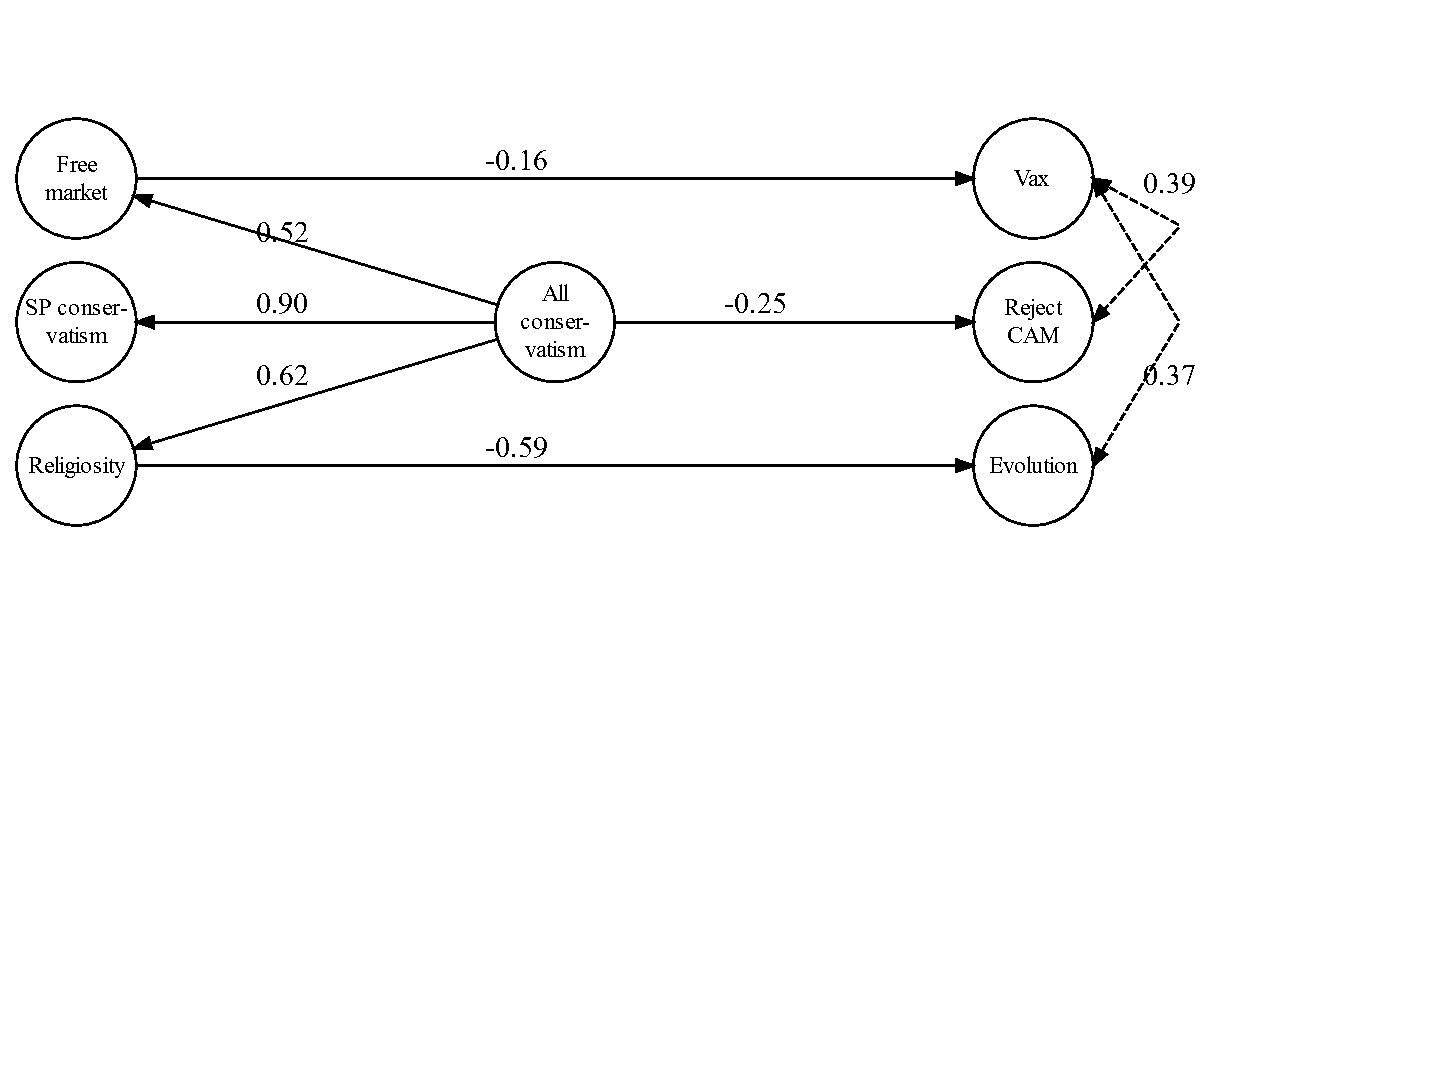
\includegraphics[width=6in]{finalpolSEM.pdf} \\
\raisebox{2.8in}{\bf \helv{b}} & 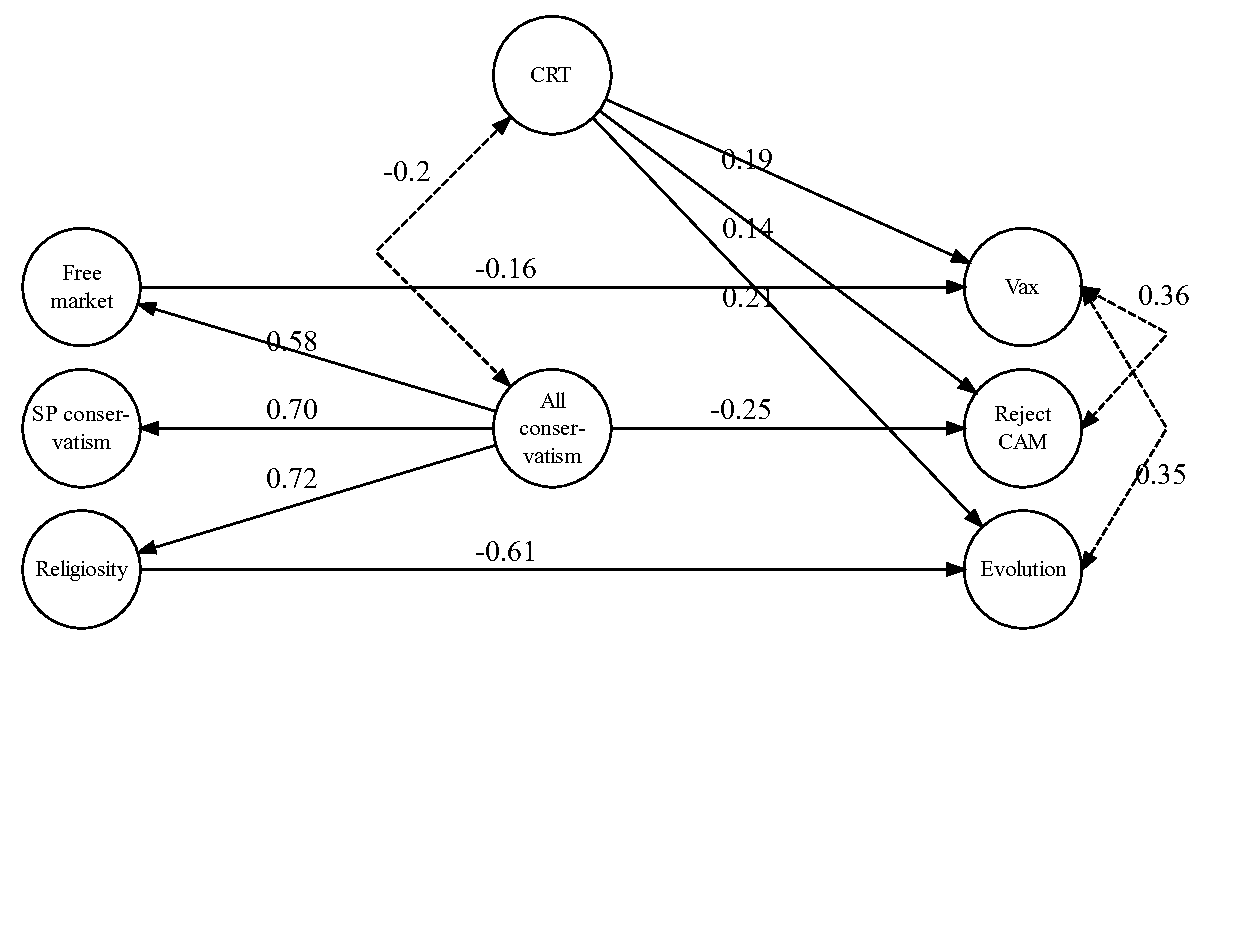
\includegraphics[width=6in]{superSEM.pdf}
\end{tabular}
\end{center}
	\caption{Structural equation model to predict scientific attitudes. 
		Panel a shows the model with the three worldview constructs as predictors.
		Panel b shows the same model after inclusion of a factor representing CRT performance.
		All links and correlations shown are 
		standardized and significant; all $p \leq .05$. Dashed lines indicate correlations between latent variables.
		Indicator variables and their loadings, and disturbances on endogenous factors are not
		shown. Links between latent variables that are not shown are 
		constrained to zero. 
		Loadings and variances of single-indicator latent 
		variables are reported in Tables~\ref{tab:indicatormodels}
		and~\ref{tab:descriptives}.}
	\label{fig:finalpolSEM}
\end{figure}

The model captures the correlations between the three scientific constructs (although 
unlike for the first-order correlations in Table~\ref{tab:lvcor}, 
CAM rejection
was not significantly correlated with evolution). 
This replicates other findings that people's attitudes towards scientific issues often covary \cite<e.g.,>{Lewandowsky12a}. 
Accordingly, one or more aspects of conservatism uniformly predicted reduced acceptance of scientific issues.
The All conservatism factor was found to be negatively associated with rejection of CAM, suggesting that people with 
conservative worldviews
are more likely to accept CAM. The All conservatism factor was not associated with the remaining two scientific themes. Instead, it was the sub-components
of overall conservatism that predicted rejection of those other issues. Rejection of vaccinations is predicted exclusively by free-market endorsement and rejection of evolution 
by religiosity. 
This model shows that rejection of science is not simply driven by a general left-right dimension of political orientation. 
Our more differentiated assessment of worldview helped us 
identify relevant sub-dimensions of the overall cluster of worldviews, 
which differentially influence people's acceptance or rejection of scientific propositions.
Crucially, however, the polarity of the effects was uniform across issues, with no evidence that people on the political
left were less inclined to accept scientific issues.

We next expanded this model by adding CRT performance as a further predictor but clamping 
the regression estimates to their values from the original model. 
This expanded model is shown in panel b of Figure~\ref{fig:finalpolSEM} and, notwithstanding the imposition
of strong constraints,
it fit acceptably well, 
$\chi^2(26)=113.86$; 
SRMR=0.064; CFI=0.951; 
RMSEA=0.058 (90\% CI:
0.047--
0.069).
The uniformly positive weights between CRT performance and endorsement of science again
replicate earlier results \cite{Shtulman14,WagnerEgger18} and confirm that the
first-order correlations in Table~\ref{tab:lvcor} stand up to the inclusion of all worldview-related constructs.

\subsubsection{Predicting attitudes towards gender equality}
We developed a parallel hierarchical model to predict attitudes towards the gender-related constructs from the same set of worldview constructs.
The model is shown in Figure~\ref{fig:genderSEM} and fit very well,
$\chi^2(5)=20.45$; 
SRMR=0.032; CFI=0.985; 
RMSEA=0.055 (90\% CI:
0.032--
0.081).
The model shows that the All conservatism factor predicted all aspects of gender attitudes in the expected direction: greater
conservatism predicted less endorsement of the idea that men and women are equal, and it predicted greater acceptance of
evolved or natural differences between men and women. In addition, religiosity uniquely predicted rejection of the idea that men and
women evolved differently, thus again dissociating between different aspects of overall conservatism.
\begin{figure}[tp] %fig:genderSEM
\fitfigure{finalgenderSEM.pdf}
\caption{Structural equation model to predict gender attitudes from worldviews. 
	All links and correlations shown are 
	standardized and significant; all $p \leq .05$. Dashed lines indicate correlations between latent variables.
	Indicator variables and their loadings, and disturbances on endogenous factors are not
	shown. Links between latent variables that are not shown are 
	constrained to zero. 
	Loadings and variances of single-indicator latent 
	variables are reported in Tables~\ref{tab:indicatormodels}
	and~\ref{tab:descriptives}.}
\label{fig:genderSEM}
\end{figure}

\subsection{Nurture vs. nature vs. evolution}
The final analysis considered the relationship between people's
acceptance of evolution and the 
constructs that probed the origins and extent of gender differences. 
This analysis therefore explored the dilemmas postulated in 
Figure~\ref{fig:dilemmas}.
We divided participants according to their political views,
conducting a median split of the composite scores on the 
socio-political conservatism scale.
Figure~\ref{fig:conslibevogrid} illustrates the results,
using composite scores for all constructs, with liberals shown
on the left and conservatives on the right. 

The top row of panels 
illustrates the putative dilemma confronting conservatives. 
The panels plot
the two constructs concerning the origin of gender differences (men and women evolved
differently [abscissa] vs. men and women are naturally different [ordinate]).
The color of plotting symbols shows attitudes towards evolution, with dark
dots indicating rejection and light dots acceptance.
Several observations can be made:
First, the two constructs for the origins of gender differences are highly
correlated irrespective of political views.
Second, conservatives are more likely overall to think that
men and women differ naturally than liberals. 
Third, as expected from the pattern of correlations in 
Table~\ref{tab:compcor}, more conservatives
than liberals reject Darwinian evolution (more dark points on the right). 
Crucially, conservatives
who reject evolution also tend to endorse gender differences---however,
as revealed by the cluster of dark points in the top left, that endorsement mainly involves the idea that men and women are
somehow ``naturally'' different, rather than the idea that they
``evolved differently.'' Conservatives thus
resolved their dilemma by ascribing gender differences to unspecified
natural factors while rejecting evolution both generally and specifically with respect to gender differences.

\begin{figure}[tp] %fig:conslibevogrid
\fitfigure{conslibequalitygridAll.pdf}
\caption{Relationship between the three gender-related
	constructs and acceptance of evolution.
	Liberals are shown on the left and conservatives on the right (median split of socio-political conservatism construct).
	The top panels show
	acceptance of evolution (represented by color
of plotting symbols) and people's responses to the constructs probing the
origin of gender differences. 
	The bottom panels show belief in gender equality (represented by
color of plotting symbols) and people's responses to the two constructs probing evolution generally (ordinate) and that men and women evolved differently (abscissa).
Composite scores are used for all constructs.
Dashed horizontal and vertical lines represent marginal
means. Points are randomly jittered to reduce over-printing.}
\label{fig:conslibevogrid}
\end{figure}

The bottom row of panels illustrates the putative dilemma facing 
liberals. 
The panels plot
the two constructs probing evolution, with gender differences (men and women evolved
differently) on the abscissa, and general evolution acceptance on the ordinate. The color of plotting symbols shows attitudes towards 
gender equality, with darker points representing greater endorsement
of equality.
It is clear that more liberals than conservatives endorse evolution
and that liberals are more inclined to endorse gender equality (dots are generally darker in the left panel).
Crucially, a large number of liberals accept evolution 
and gender equality---however,
as revealed by the cluster of dark points in the top left, 
that endorsement is accompanied by a reduced belief 
in the evolution of gender differences.
Liberals thus
resolved their dilemma by rejecting the evolution of
gender differences while embracing evolution generally together with
equality.

\section{Discussion}
\subsection{Relationship to previous results}
Our results coordinate well with multiple precedents in the literature,
which we take up for each of the
constructs examined. 
Considering first religiosity, we replicated 
the substantial association between stronger religious beliefs
and conservatism in the American population \cite{Malka12,Schlenker12}. 
In our
study this association generalized across a broadly-defined socio-political 
conservatism construct as well as a specific construct
targeting endorsement of laissez-faire free-market economics.
We also replicated the long-standing strong negative
association between religiosity and acceptance of evolution \cite<e.g.,>{Ecklund17,Tom18} 
and the
modest negative association between religiosity and analytic thinking
(i.e., CRT performance) reported previously \cite{Jack16,Shenhav12,Stagnaro19}.
Likewise, the correlations between religiosity and the gender
constructs (e.g., Table~\ref{tab:lvcor}) are consistent 
with previous reports that religiosity predicts sexism \cite{VanAssche19}.
Our results go beyond previous findings because our
scales did not probe discriminatory sexism but the origin of presumed
gender differences. We find that religiosity makes it less likely that
people believe that gender differences have evolved.

The negative association between religiosity and CAM rejection 
is also unsurprising 
in light of previous research that has shown acceptance of CAM 
to be driven by intuitive thinking, paranormal beliefs,
and ontological confusions \cite{Lindeman11}.
At least one of those variables (intuitive thinking)
is also known to be a predictor of religiosity \cite<e.g.,>{Shenhav12}.
The positive correlation between CAM rejection and
acceptance of vaccinations 
replicates much previous research \cite<e.g.,>{Attwell18,Browne15,Bryden18,Ernst02}.

However, our findings concerning religiosity also deviate from aspects
of other recent research
\cite{Rutjens17}. 
Unlike \citeauthor{Rutjens17}, we 
found no evidence of a link
between religiosity and rejection of vaccinations. 
Given that  \citeauthor{Rutjens17} observed this link
only in some of their studies and only for some measures
of religiosity (mainly measures of religious orthodoxy),
we are not concerned about this apparent 
departure from previous results. Indeed, in another
recent as-yet unpublished study involving identical constructs, 
we did observe
a negative association between vaccination and religiosity, 
suggesting that this relationship may well be real but is only
observable in certain circumstances.

Turning to the associations involving CRT performance, the observed 
modest but significant negative correlation with
religiosity replicates previous results \cite{Gervais12a,Shenhav12,Stagnaro19}. 
\citeA{Jost17} reported a 
meta analysis of 13 studies that related CRT performance to political views.
The vast majority of those studies showed
that liberals exhibited more cognitive reflection than conservatives.
In the present data, this is echoed by the modest negative
correlation with free market, although it was not reflected in the
socio-political conservatism measure. 
The positive associations of the CRT with endorsement of all three
scientific constructs, vaccination, CAM rejection, and evolution
replicate similar previous findings \cite{Shtulman14,WagnerEgger18}.
The association also coordinates well with recent findings that analytical thinking
is associated with better differentiation between ``fake news'' and
valid information \cite{Pennycook18}. 

\subsection{Rejection of science on the political left?}
Our findings provide 
little or no evidence that people on the 
political left reject vaccinations. 
On the contrary, to the extent that 
worldviews determined vaccination attitudes, it was free-market endorsement that
predicted rejection. 
This result 
parallels a similar association observed by \citeA{Hornsey18},
albeit using a different instrument to measure Libertarian
attidudes (hierarchical-individualism as opposed to free-market endorsement).
The result 
is also consonant with the notion that libertarians object to the
government intrusion arising from mandatory vaccination programs
\cite{Kahan10a}. It also meshes well with the pattern 
observed by \citeA{Lewandowsky13b}, who showed that when
socio-political conservatism was removed from a model, 
free-market endorsement on its own predicted rejection
of vaccinations (whereas the converse was not true).
Overall, our results thus converge with other recent findings
that have found an association between right-wing politics and
rejection of vaccinations \cite{Baumgaertner18,Kahan10a,Rabinowitz16}.
In a recent cross-sectional analysis of voting behavior and 
vaccination rates across 
European countries, \citeA{Kennedy19} found a strong
relationship between the vote share for populist parties 
and vaccine hesitancy. 

Similarly, contrary to reports that CAM use and left-wing ideas 
have a natural affinity for each other \cite<see, e.g.,>{Keshet09},
we found that
CAM rejection was negatively, but modestly, associated with 
the All conservatism factor that subsumed
all three of our worldview constructs; namely, religiosity, 
free market endorsement, and socio-political conservatism. 
Moreover, in our data, none of the gender
constructs were associated with CAM attitudes. This
runs counter to the idea that CAM use 
is ``feminist'' \cite{Scott98a}.
To our knowledge, our results constitute 
the first empirical examination of the links
between political
views and CAM attitudes. 
Our results that conservatives are more likely to embrace
CAM is consonant with 
historical analyses that have found strong links
between right-wing organizations, such as the
John Birch Society in the U.S., and endorsement
of ``alternative'' cancer treatments \cite{Markle78}.
The present result adds to the list of failed attempts
to discover science denial on the political left
\cite<e.g.,>{Hamilton11,Hamilton15c,Hamilton15a,Hamilton15b,Kahan10a,Lewandowsky13b,Tom18}. 

\subsection{Attitudes towards gender differences}
We observed an intriguing 
interplay of the attitudes towards general Darwinian evolution,
gender differences, and how those gender differences
might have arisen.
At a coarse level of analysis, we
observed three unsurprising associations: The idea that 
men and women differ naturally was highly 
correlated with the idea that they evolved differently, but
was negatively correlated with
the construct that proclaimed gender equality. 
The equality construct was 
also negatively
correlated with the idea that men and women evolved differently,
although that correlation was smaller than for 
natural differences. 

At a more detailed level of analysis, several
intriguing associations emerged.
First, acceptance of general Darwinian evolution was 
positively associated with two seemingly conflicting constructs; 
namely, that men and women evolved differently \textit{and} that they are
the same. Moreover, evolution was negatively correlated with the idea
that men and women are naturally different, even though evolution
is one way in which such ``natural'' differences might have emerged.
A similarly nuanced  pattern obtained when the 
worldview constructs were used to predict 
gender attitudes. Although the over-arching All conservatism
factor functioned as expected, with negative weights for gender equality 
and positive weights for the two constructs insisting on
gender differences, 
there was an additional selective effect of religiosity on 
the rejection of evolved gender differences.

Further analysis revealed that the involvement of evolution, 
either on its own or in explaining
gender differences, served as a ``wedge issue'' that disrupted
otherwise straightforward associations between right-wing politics
and opposition to gender equality (and, vice versa, rejection of
gender differences and left-wing politics) and---as foreshadowed
in Figure~\ref{fig:dilemmas}---created 
dilemmas for participants of all political persuasions.
As noted in connection with
Figure~\ref{fig:conslibevogrid},
conservatives who strongly
rejected Darwinian evolution resolved their dilemma by 
endorsing 
``natural'' gender differences while rejecting
evolved gender differences. Those participants were
thus willing to forego endorsement of gender differences to maintain
consistency with their opposition to evolution. 
Conversely, liberals who are strongly committed to gender equality
tend to reject the idea of evolved gender differences, even though
those participants are demonstrably committed to accepting evolution.
Those 
participants were
thus willing to forego endorsement of a specific manifestation of evolution
to maintain
consistency with their commitment to equality.
Thus, partisans of either stripe can agree in their rejection of the idea that men and
women evolved differently, but they do so for entirely different
reasons. Conservatives do so when they are committed to reject evolution, and liberal do 
so when they are committed to gender equality. Both groups therefore resolve the dilemmas
posed by our gender constructs by ``sacrificing'' endorsement of evolved gender
differences.

\section{Conclusion}
Our results contribute to two seemingly conflicting streams 
of outcomes in the literature on 
how worldviews moderate people's responses to scientific issues. 
On the one hand, there is much evidence for pervasive attitudinal
asymmetry, at least in the United States, with conservatives 
being more likely to reject
well-established scientific propositions than liberals. To date,
little or no evidence for left-wing science denial has been reported.
We add to this stream by showing that, contrary to previous largely
anecdotal reports, liberals are more likely to reject complementary
and alternative medicines, in line with the scientific evidence, than
conservatives. 

On the other hand, there is considerable evidence that
liberals and conservatives \textit{process} scientific data
in a symmetrical fashion. That is, liberals and conservatives
alike resort to the same cognitive shortcuts when data conform to their
biases, giving rise to a symmetric set of errors \cite{Kahan17b,Washburn17}.
We also add to this stream of research by showing that, when confronted
by worldview-triggered dilemmas, both liberals and conservatives
resolve those dilemmas in an equally ``rational'' fashion,
by selectively ``sacrificing'' endorsement of a specific
construct about gender differences. 
Liberals, who generally endorse evolution, believe that for 
some reason it did not affect differences between the sexes; 
this could be rationalized perhaps by assuming that evolution causes 
differences only between but not within species. 
Conservatives, who frequently reject evolution, believe that men and women differ 
naturally without having evolved differently; this could be 
rationalized by assuming, for instance, that those natural differences 
were the result of divine intervention.

A final contribution of our study is that it points to the advantages
of a more nuanced analysis of political worldviews, beyond a convenient
but simplistic classification of people into left and right, or liberals
and conservatives. While this classification is sufficient
to explain some scientific attitudes---for example, it matters
little how one measures political worldviews to explain
rejection of climate science \cite<e.g.,>{Hornsey16,Kahan15}---there
are other circumstances in which a more nuanced differentiation
between different aspects of worldviews provides considerably 
greater explanatory power.

%\bibliography{mega,megaIPsub}
\begin{thebibliography}{}
	
	\bibitem [\protect \citeauthoryear {%
		Allum%
		, Sturgis%
		, Tabourazi%
		\BCBL {}\ \BBA {} Brunton-Smith%
	}{%
		Allum%
		\ \protect \BOthers {.}}{%
		{\protect \APACyear {2008}}%
	}]{%
		Allum08}
	\APACinsertmetastar {%
		Allum08}%
	\begin{APACrefauthors}%
		Allum, N.%
		, Sturgis, P.%
		, Tabourazi, D.%
		\BCBL {}\ \BBA {} Brunton-Smith, I.%
	\end{APACrefauthors}%
	\unskip\
	\newblock
	\APACrefYearMonthDay{2008}{}{}.
	\newblock
	{\BBOQ}\APACrefatitle {Science knowledge and attitudes across cultures: a
		meta-analysis} {Science knowledge and attitudes across cultures: a
		meta-analysis}.{\BBCQ}
	\newblock
	\APACjournalVolNumPages{Public Understanding of Science}{17}{}{35--54}.
	\newblock
	\begin{APACrefDOI} \doi{10.1177/0963662506070159} \end{APACrefDOI}
	\PrintBackRefs{\CurrentBib}
	
	\bibitem [\protect \citeauthoryear {%
		Anderson%
		\ \BBA {} Peters%
	}{%
		Anderson%
		\ \BBA {} Peters%
	}{%
		{\protect \APACyear {2016}}%
	}]{%
		Anderson16}
	\APACinsertmetastar {%
		Anderson16}%
	\begin{APACrefauthors}%
		Anderson, K.%
		\BCBT {}\ \BBA {} Peters, G.%
	\end{APACrefauthors}%
	\unskip\
	\newblock
	\APACrefYearMonthDay{2016}{}{}.
	\newblock
	{\BBOQ}\APACrefatitle {The trouble with negative emissions} {The trouble with
		negative emissions}.{\BBCQ}
	\newblock
	\APACjournalVolNumPages{Science}{354}{6309}{182--183}.
	\newblock
	\begin{APACrefDOI} \doi{10.1126/science.aah4567} \end{APACrefDOI}
	\PrintBackRefs{\CurrentBib}
	
	\bibitem [\protect \citeauthoryear {%
		Attwell%
		, Ward%
		, Meyer%
		, Rokkas%
		\BCBL {}\ \BBA {} Leask%
	}{%
		Attwell%
		\ \protect \BOthers {.}}{%
		{\protect \APACyear {2018}}%
	}]{%
		Attwell18}
	\APACinsertmetastar {%
		Attwell18}%
	\begin{APACrefauthors}%
		Attwell, K.%
		, Ward, P\BPBI R.%
		, Meyer, S\BPBI B.%
		, Rokkas, P\BPBI J.%
		\BCBL {}\ \BBA {} Leask, J.%
	\end{APACrefauthors}%
	\unskip\
	\newblock
	\APACrefYearMonthDay{2018}{}{}.
	\newblock
	{\BBOQ}\APACrefatitle {``{D}o-it-yourself'': {V}accine rejection and
		complementary and alternative medicine ({CAM})} {``{D}o-it-yourself'':
		{V}accine rejection and complementary and alternative medicine
		({CAM})}.{\BBCQ}
	\newblock
	\APACjournalVolNumPages{Social Science \& Medicine}{196}{}{106--114}.
	\newblock
	\begin{APACrefDOI} \doi{10.1016/j.socscimed.2017.11.022} \end{APACrefDOI}
	\PrintBackRefs{\CurrentBib}
	
	\bibitem [\protect \citeauthoryear {%
		Baumgaertner%
		, Carlisle%
		\BCBL {}\ \BBA {} Justwan%
	}{%
		Baumgaertner%
		\ \protect \BOthers {.}}{%
		{\protect \APACyear {2018}}%
	}]{%
		Baumgaertner18}
	\APACinsertmetastar {%
		Baumgaertner18}%
	\begin{APACrefauthors}%
		Baumgaertner, B.%
		, Carlisle, J\BPBI E.%
		\BCBL {}\ \BBA {} Justwan, F.%
	\end{APACrefauthors}%
	\unskip\
	\newblock
	\APACrefYearMonthDay{2018}{}{}.
	\newblock
	{\BBOQ}\APACrefatitle {The influence of political ideology and trust on
		willingness to vaccinate} {The influence of political ideology and trust on
		willingness to vaccinate}.{\BBCQ}
	\newblock
	\APACjournalVolNumPages{{PLOS} {ONE}}{13}{}{e0191728}.
	\newblock
	\begin{APACrefDOI} \doi{10.1371/journal.pone.0191728} \end{APACrefDOI}
	\PrintBackRefs{\CurrentBib}
	
	\bibitem [\protect \citeauthoryear {%
		Bentler%
		\ \BBA {} Chou%
	}{%
		Bentler%
		\ \BBA {} Chou%
	}{%
		{\protect \APACyear {1987}}%
	}]{%
		Bentler87}
	\APACinsertmetastar {%
		Bentler87}%
	\begin{APACrefauthors}%
		Bentler, P\BPBI M.%
		\BCBT {}\ \BBA {} Chou, C\BHBI P.%
	\end{APACrefauthors}%
	\unskip\
	\newblock
	\APACrefYearMonthDay{1987}{}{}.
	\newblock
	{\BBOQ}\APACrefatitle {Practical Issues in Structural Modeling} {Practical
		issues in structural modeling}.{\BBCQ}
	\newblock
	\APACjournalVolNumPages{Sociological Methods \& Research}{16}{}{78--117}.
	\PrintBackRefs{\CurrentBib}
	
	\bibitem [\protect \citeauthoryear {%
		Browne%
		, Thomson%
		, Rockloff%
		\BCBL {}\ \BBA {} Pennycook%
	}{%
		Browne%
		\ \protect \BOthers {.}}{%
		{\protect \APACyear {2015}}%
	}]{%
		Browne15}
	\APACinsertmetastar {%
		Browne15}%
	\begin{APACrefauthors}%
		Browne, M.%
		, Thomson, P.%
		, Rockloff, M\BPBI J.%
		\BCBL {}\ \BBA {} Pennycook, G.%
	\end{APACrefauthors}%
	\unskip\
	\newblock
	\APACrefYearMonthDay{2015}{}{}.
	\newblock
	{\BBOQ}\APACrefatitle {Going against the Herd: Psychological and Cultural
		Factors Underlying the `Vaccination Confidence Gap'} {Going against the herd:
		Psychological and cultural factors underlying the `vaccination confidence
		gap'}.{\BBCQ}
	\newblock
	\APACjournalVolNumPages{{PLOS} {ONE}}{10}{}{e0132562}.
	\newblock
	\begin{APACrefDOI} \doi{10.1371/journal.pone.0132562} \end{APACrefDOI}
	\PrintBackRefs{\CurrentBib}
	
	\bibitem [\protect \citeauthoryear {%
		Bryden%
		, Browne%
		, Rockloff%
		\BCBL {}\ \BBA {} Unsworth%
	}{%
		Bryden%
		\ \protect \BOthers {.}}{%
		{\protect \APACyear {2018}}%
	}]{%
		Bryden18}
	\APACinsertmetastar {%
		Bryden18}%
	\begin{APACrefauthors}%
		Bryden, G\BPBI M.%
		, Browne, M.%
		, Rockloff, M.%
		\BCBL {}\ \BBA {} Unsworth, C.%
	\end{APACrefauthors}%
	\unskip\
	\newblock
	\APACrefYearMonthDay{2018}{}{}.
	\newblock
	{\BBOQ}\APACrefatitle {Anti-vaccination and pro-{CAM} attitudes both reflect
		magical beliefs about health} {Anti-vaccination and pro-{CAM} attitudes both
		reflect magical beliefs about health}.{\BBCQ}
	\newblock
	\APACjournalVolNumPages{Vaccine}{36}{}{1227--1234}.
	\newblock
	\begin{APACrefDOI} \doi{10.1016/j.vaccine.2017.12.068} \end{APACrefDOI}
	\PrintBackRefs{\CurrentBib}
	
	\bibitem [\protect \citeauthoryear {%
		Buss%
	}{%
		Buss%
	}{%
		{\protect \APACyear {1989}}%
	}]{%
		Buss89}
	\APACinsertmetastar {%
		Buss89}%
	\begin{APACrefauthors}%
		Buss, D\BPBI M.%
	\end{APACrefauthors}%
	\unskip\
	\newblock
	\APACrefYearMonthDay{1989}{}{}.
	\newblock
	{\BBOQ}\APACrefatitle {Sex differences in human mate preferences:
		{E}volutionary hypotheses tested in 37 cultures} {Sex differences in human
		mate preferences: {E}volutionary hypotheses tested in 37 cultures}.{\BBCQ}
	\newblock
	\APACjournalVolNumPages{Behavioral and Brain Sciences}{12}{}{1--49}.
	\PrintBackRefs{\CurrentBib}
	
	\bibitem [\protect \citeauthoryear {%
		Buss%
	}{%
		Buss%
	}{%
		{\protect \APACyear {1996}}%
	}]{%
		Buss96}
	\APACinsertmetastar {%
		Buss96}%
	\begin{APACrefauthors}%
		Buss, D\BPBI M.%
	\end{APACrefauthors}%
	\unskip\
	\newblock
	\APACrefYearMonthDay{1996}{}{}.
	\newblock
	{\BBOQ}\APACrefatitle {Sexual conflict: Evolutionary insights into feminism and
		the “battle of the sexes.”} {Sexual conflict: Evolutionary insights into
		feminism and the “battle of the sexes.”}.{\BBCQ}
	\newblock
	\BIn{} D\BPBI M.~Buss\ \BBA {} N.~Malamuth\ (\BEDS), \APACrefbtitle {Sex,
		power, conflict: Evolutionary and feminist perspectives} {Sex, power,
		conflict: Evolutionary and feminist perspectives}\ (\BPGS\ 296--318).
	\newblock
	\APACaddressPublisher{}{Oxford University Press}.
	\PrintBackRefs{\CurrentBib}
	
	\bibitem [\protect \citeauthoryear {%
		Buss%
		, Shackelford%
		, Kirkpatrick%
		\BCBL {}\ \BBA {} Larsen%
	}{%
		Buss%
		\ \protect \BOthers {.}}{%
		{\protect \APACyear {2001}}%
	}]{%
		Buss01}
	\APACinsertmetastar {%
		Buss01}%
	\begin{APACrefauthors}%
		Buss, D\BPBI M.%
		, Shackelford, T\BPBI K.%
		, Kirkpatrick, L\BPBI A.%
		\BCBL {}\ \BBA {} Larsen, R\BPBI J.%
	\end{APACrefauthors}%
	\unskip\
	\newblock
	\APACrefYearMonthDay{2001}{}{}.
	\newblock
	{\BBOQ}\APACrefatitle {A Half Century of Mate Preferences: The Cultural
		Evolution of Values} {A half century of mate preferences: The cultural
		evolution of values}.{\BBCQ}
	\newblock
	\APACjournalVolNumPages{Journal of Marriage and Family}{63}{}{491--503}.
	\newblock
	\begin{APACrefDOI} \doi{10.1111/j.1741-3737.2001.00491.x} \end{APACrefDOI}
	\PrintBackRefs{\CurrentBib}
	
	\bibitem [\protect \citeauthoryear {%
		Cain%
	}{%
		Cain%
	}{%
		{\protect \APACyear {1989}}%
	}]{%
		Cain89}
	\APACinsertmetastar {%
		Cain89}%
	\begin{APACrefauthors}%
		Cain, P\BPBI A.%
	\end{APACrefauthors}%
	\unskip\
	\newblock
	\APACrefYearMonthDay{1989}{}{}.
	\newblock
	{\BBOQ}\APACrefatitle {Feminism and the Limits of Equality} {Feminism and the
		limits of equality}.{\BBCQ}
	\newblock
	\APACjournalVolNumPages{Georgia Law Review}{24}{}{803 -- 847}.
	\PrintBackRefs{\CurrentBib}
	
	\bibitem [\protect \citeauthoryear {%
		Castagno%
	}{%
		Castagno%
	}{%
		{\protect \APACyear {2017}}%
	}]{%
		Castagno17}
	\APACinsertmetastar {%
		Castagno17}%
	\begin{APACrefauthors}%
		Castagno, A\BPBI E.%
	\end{APACrefauthors}%
	\unskip\
	\newblock
	\APACrefYearMonthDay{2017}{}{}.
	\newblock
	{\BBOQ}\APACrefatitle {Liberal Ideologies and Federal School Reform: Following
		Individualism, Meliorism, and Neutrality Through {SIG} Policy to Adelante
		Alternative School} {Liberal ideologies and federal school reform: Following
		individualism, meliorism, and neutrality through {SIG} policy to adelante
		alternative school}.{\BBCQ}
	\newblock
	\APACjournalVolNumPages{Urban Education}{}{}{}.
	\newblock
	\begin{APACrefDOI} \doi{10.1177/0042085916685762} \end{APACrefDOI}
	\PrintBackRefs{\CurrentBib}
	
	\bibitem [\protect \citeauthoryear {%
		Coffman%
		\ \BBA {} MacCallum%
	}{%
		Coffman%
		\ \BBA {} MacCallum%
	}{%
		{\protect \APACyear {2005}}%
	}]{%
		Coffman05}
	\APACinsertmetastar {%
		Coffman05}%
	\begin{APACrefauthors}%
		Coffman, D\BPBI L.%
		\BCBT {}\ \BBA {} MacCallum, R\BPBI C.%
	\end{APACrefauthors}%
	\unskip\
	\newblock
	\APACrefYearMonthDay{2005}{}{}.
	\newblock
	{\BBOQ}\APACrefatitle {Using Parcels to Convert Path Analysis Models Into
		Latent Variable Models} {Using parcels to convert path analysis models into
		latent variable models}.{\BBCQ}
	\newblock
	\APACjournalVolNumPages{Multivariate Behavioral Research}{40}{}{235--259}.
	\PrintBackRefs{\CurrentBib}
	
	\bibitem [\protect \citeauthoryear {%
		Eagly%
	}{%
		Eagly%
	}{%
		{\protect \APACyear {2018}}%
	}]{%
		Eagly18}
	\APACinsertmetastar {%
		Eagly18}%
	\begin{APACrefauthors}%
		Eagly, A\BPBI H.%
	\end{APACrefauthors}%
	\unskip\
	\newblock
	\APACrefYearMonthDay{2018}{}{}.
	\newblock
	{\BBOQ}\APACrefatitle {The Shaping of Science by Ideology: How Feminism
		Inspired, Led, and Constrained Scientific Understanding of Sex and Gender}
	{The shaping of science by ideology: How feminism inspired, led, and
		constrained scientific understanding of sex and gender}.{\BBCQ}
	\newblock
	\APACjournalVolNumPages{Journal of Social Issues}{74}{}{871--888}.
	\newblock
	\begin{APACrefDOI} \doi{10.1111/josi.12291} \end{APACrefDOI}
	\PrintBackRefs{\CurrentBib}
	
	\bibitem [\protect \citeauthoryear {%
		Eagly%
		\ \BBA {} Wood%
	}{%
		Eagly%
		\ \BBA {} Wood%
	}{%
		{\protect \APACyear {2013}}%
	}]{%
		Eagly13}
	\APACinsertmetastar {%
		Eagly13}%
	\begin{APACrefauthors}%
		Eagly, A\BPBI H.%
		\BCBT {}\ \BBA {} Wood, W.%
	\end{APACrefauthors}%
	\unskip\
	\newblock
	\APACrefYearMonthDay{2013}{}{}.
	\newblock
	{\BBOQ}\APACrefatitle {The Nature{\textendash}Nurture Debates} {The
		nature{\textendash}nurture debates}.{\BBCQ}
	\newblock
	\APACjournalVolNumPages{Perspectives on Psychological Science}{8}{}{340--357}.
	\newblock
	\begin{APACrefDOI} \doi{10.1177/1745691613484767} \end{APACrefDOI}
	\PrintBackRefs{\CurrentBib}
	
	\bibitem [\protect \citeauthoryear {%
		Ecklund%
		, Scheitle%
		, Peifer%
		\BCBL {}\ \BBA {} Bolger%
	}{%
		Ecklund%
		\ \protect \BOthers {.}}{%
		{\protect \APACyear {2017}}%
	}]{%
		Ecklund17}
	\APACinsertmetastar {%
		Ecklund17}%
	\begin{APACrefauthors}%
		Ecklund, E\BPBI H.%
		, Scheitle, C\BPBI P.%
		, Peifer, J.%
		\BCBL {}\ \BBA {} Bolger, D.%
	\end{APACrefauthors}%
	\unskip\
	\newblock
	\APACrefYearMonthDay{2017}{}{}.
	\newblock
	{\BBOQ}\APACrefatitle {Examining Links Between Religion, Evolution Views, and
		Climate Change Skepticism} {Examining links between religion, evolution
		views, and climate change skepticism}.{\BBCQ}
	\newblock
	\APACjournalVolNumPages{Environment and Behavior}{49}{}{985--1006}.
	\newblock
	\begin{APACrefDOI} \doi{10.1177/0013916516674246} \end{APACrefDOI}
	\PrintBackRefs{\CurrentBib}
	
	\bibitem [\protect \citeauthoryear {%
		Ernst%
	}{%
		Ernst%
	}{%
		{\protect \APACyear {2002}}%
	}]{%
		Ernst02}
	\APACinsertmetastar {%
		Ernst02}%
	\begin{APACrefauthors}%
		Ernst, E.%
	\end{APACrefauthors}%
	\unskip\
	\newblock
	\APACrefYearMonthDay{2002}{}{}.
	\newblock
	{\BBOQ}\APACrefatitle {Rise in popularity of complementary and alternative
		medicine: reasons and consequences for vaccination} {Rise in popularity of
		complementary and alternative medicine: reasons and consequences for
		vaccination}.{\BBCQ}
	\newblock
	\APACjournalVolNumPages{Vaccine}{20}{}{S90--S93}.
	\newblock
	\begin{APACrefDOI} \doi{10.1016/S0264-410X(01)00290-0} \end{APACrefDOI}
	\PrintBackRefs{\CurrentBib}
	
	\bibitem [\protect \citeauthoryear {%
		Everett%
	}{%
		Everett%
	}{%
		{\protect \APACyear {2013}}%
	}]{%
		Everett13}
	\APACinsertmetastar {%
		Everett13}%
	\begin{APACrefauthors}%
		Everett, J\BPBI A.%
	\end{APACrefauthors}%
	\unskip\
	\newblock
	\APACrefYearMonthDay{2013}{}{}.
	\newblock
	{\BBOQ}\APACrefatitle {The 12 Item Social and Economic Conservatism Scale
		{(SECS)}} {The 12 item social and economic conservatism scale
		{(SECS)}}.{\BBCQ}
	\newblock
	\APACjournalVolNumPages{PLOS ONE}{8}{}{e82131}.
	\newblock
	\begin{APACrefDOI} \doi{10.1371/journal.pone.0082131} \end{APACrefDOI}
	\PrintBackRefs{\CurrentBib}
	
	\bibitem [\protect \citeauthoryear {%
		Fine%
	}{%
		Fine%
	}{%
		{\protect \APACyear {2013}}%
	}]{%
		Fine13}
	\APACinsertmetastar {%
		Fine13}%
	\begin{APACrefauthors}%
		Fine, C.%
	\end{APACrefauthors}%
	\unskip\
	\newblock
	\APACrefYearMonthDay{2013}{}{}.
	\newblock
	{\BBOQ}\APACrefatitle {Is There Neurosexism in Functional Neuroimaging
		Investigations of Sex Differences?} {Is there neurosexism in functional
		neuroimaging investigations of sex differences?}{\BBCQ}
	\newblock
	\APACjournalVolNumPages{Neuroethics}{6}{}{369--409}.
	\newblock
	\begin{APACrefDOI} \doi{10.1007/s12152-012-9169-1} \end{APACrefDOI}
	\PrintBackRefs{\CurrentBib}
	
	\bibitem [\protect \citeauthoryear {%
		Fine%
		, Joel%
		, Jordan-Young%
		, Kaiser~Trujillo%
		\BCBL {}\ \BBA {} Rippon%
	}{%
		Fine%
		\ \protect \BOthers {.}}{%
		{\protect \APACyear {2014}}%
	}]{%
		Fine14}
	\APACinsertmetastar {%
		Fine14}%
	\begin{APACrefauthors}%
		Fine, C.%
		, Joel, D.%
		, Jordan-Young, R.%
		, Kaiser~Trujillo, A\BPBI C.%
		\BCBL {}\ \BBA {} Rippon, G.%
	\end{APACrefauthors}%
	\unskip\
	\newblock
	\APACrefYearMonthDay{2014}{}{}.
	\newblock
	{\BBOQ}\APACrefatitle {Why Males $\ne$ Corvettes, Females $\ne$ Volvos, and
		Scientific Criticism $\ne$ Ideology: A Response to ``Equal $\ne$ The Same:
		Sex Differences in the Human Brain'' by {L}arry {C}ahill in {C}erebrum} {Why
		males $\ne$ corvettes, females $\ne$ volvos, and scientific criticism $\ne$
		ideology: A response to ``equal $\ne$ the same: Sex differences in the human
		brain'' by {L}arry {C}ahill in {C}erebrum}.{\BBCQ}
	\newblock
	\APACjournalVolNumPages{Cerebrum: The Dana forum on brain science}{}{}{}.
	\PrintBackRefs{\CurrentBib}
	
	\bibitem [\protect \citeauthoryear {%
		Fine%
		, Jordan-Young%
		, Kaiser%
		\BCBL {}\ \BBA {} Rippon%
	}{%
		Fine%
		\ \protect \BOthers {.}}{%
		{\protect \APACyear {2013}}%
	}]{%
		Fine13a}
	\APACinsertmetastar {%
		Fine13a}%
	\begin{APACrefauthors}%
		Fine, C.%
		, Jordan-Young, R.%
		, Kaiser, A.%
		\BCBL {}\ \BBA {} Rippon, G.%
	\end{APACrefauthors}%
	\unskip\
	\newblock
	\APACrefYearMonthDay{2013}{}{}.
	\newblock
	{\BBOQ}\APACrefatitle {Plasticity, plasticity, plasticity{\ldots}and the rigid
		problem of sex} {Plasticity, plasticity, plasticity{\ldots}and the rigid
		problem of sex}.{\BBCQ}
	\newblock
	\APACjournalVolNumPages{Trends in Cognitive Sciences}{17}{}{550--551}.
	\newblock
	\begin{APACrefDOI} \doi{10.1016/j.tics.2013.08.010} \end{APACrefDOI}
	\PrintBackRefs{\CurrentBib}
	
	\bibitem [\protect \citeauthoryear {%
		Frederick%
	}{%
		Frederick%
	}{%
		{\protect \APACyear {2005}}%
	}]{%
		Frederick05}
	\APACinsertmetastar {%
		Frederick05}%
	\begin{APACrefauthors}%
		Frederick, S.%
	\end{APACrefauthors}%
	\unskip\
	\newblock
	\APACrefYearMonthDay{2005}{}{}.
	\newblock
	{\BBOQ}\APACrefatitle {Cognitive Reflection and Decision Making} {Cognitive
		reflection and decision making}.{\BBCQ}
	\newblock
	\APACjournalVolNumPages{The Journal of Economic Perspectives}{19}{}{25--42}.
	\PrintBackRefs{\CurrentBib}
	
	\bibitem [\protect \citeauthoryear {%
		Gale%
	}{%
		Gale%
	}{%
		{\protect \APACyear {2014}}%
	}]{%
		Gale14}
	\APACinsertmetastar {%
		Gale14}%
	\begin{APACrefauthors}%
		Gale, N.%
	\end{APACrefauthors}%
	\unskip\
	\newblock
	\APACrefYearMonthDay{2014}{}{}.
	\newblock
	{\BBOQ}\APACrefatitle {The Sociology of Traditional, Complementary and
		Alternative Medicine} {The sociology of traditional, complementary and
		alternative medicine}.{\BBCQ}
	\newblock
	\APACjournalVolNumPages{Sociology Compass}{8}{}{805--822}.
	\newblock
	\begin{APACrefDOI} \doi{10.1111/soc4.12182} \end{APACrefDOI}
	\PrintBackRefs{\CurrentBib}
	
	\bibitem [\protect \citeauthoryear {%
		Gangarosa%
		\ \protect \BOthers {.}}{%
		Gangarosa%
		\ \protect \BOthers {.}}{%
		{\protect \APACyear {1998}}%
	}]{%
		Gangarosa98}
	\APACinsertmetastar {%
		Gangarosa98}%
	\begin{APACrefauthors}%
		Gangarosa, E\BPBI J.%
		, Galazka, A\BPBI M.%
		, Wolfe, C\BPBI R.%
		, Phillips, L\BPBI M.%
		, Gangarosa, R\BPBI E.%
		, Miller, E.%
		\BCBL {}\ \BBA {} Chen, R\BPBI T.%
	\end{APACrefauthors}%
	\unskip\
	\newblock
	\APACrefYearMonthDay{1998}{}{}.
	\newblock
	{\BBOQ}\APACrefatitle {Impact of anti-vaccine movements on pertussis control:
		the untold story} {Impact of anti-vaccine movements on pertussis control: the
		untold story}.{\BBCQ}
	\newblock
	\APACjournalVolNumPages{Lancet}{351}{}{356--361}.
	\newblock
	\begin{APACrefDOI} \doi{10.1016/S0140-6736(97)04334-1} \end{APACrefDOI}
	\PrintBackRefs{\CurrentBib}
	
	\bibitem [\protect \citeauthoryear {%
		Gervais%
		\ \BBA {} Norenzayan%
	}{%
		Gervais%
		\ \BBA {} Norenzayan%
	}{%
		{\protect \APACyear {2012}}%
	}]{%
		Gervais12a}
	\APACinsertmetastar {%
		Gervais12a}%
	\begin{APACrefauthors}%
		Gervais, W\BPBI M.%
		\BCBT {}\ \BBA {} Norenzayan, A.%
	\end{APACrefauthors}%
	\unskip\
	\newblock
	\APACrefYearMonthDay{2012}{}{}.
	\newblock
	{\BBOQ}\APACrefatitle {Analytic Thinking Promotes Religious Disbelief}
	{Analytic thinking promotes religious disbelief}.{\BBCQ}
	\newblock
	\APACjournalVolNumPages{Science}{336}{}{493--496}.
	\newblock
	\begin{APACrefDOI} \doi{10.1126/science.1215647} \end{APACrefDOI}
	\PrintBackRefs{\CurrentBib}
	
	\bibitem [\protect \citeauthoryear {%
		Hamilton%
	}{%
		Hamilton%
	}{%
		{\protect \APACyear {2011}}%
	}]{%
		Hamilton11}
	\APACinsertmetastar {%
		Hamilton11}%
	\begin{APACrefauthors}%
		Hamilton, L\BPBI C.%
	\end{APACrefauthors}%
	\unskip\
	\newblock
	\APACrefYearMonthDay{2011}{}{}.
	\newblock
	{\BBOQ}\APACrefatitle {Education, politics and opinions about climate change
		evidence for interaction effects} {Education, politics and opinions about
		climate change evidence for interaction effects}.{\BBCQ}
	\newblock
	\APACjournalVolNumPages{Climatic Change}{104}{}{231--242}.
	\newblock
	\begin{APACrefDOI} \doi{10.1007/s10584-010-9957-8} \end{APACrefDOI}
	\PrintBackRefs{\CurrentBib}
	
	\bibitem [\protect \citeauthoryear {%
		Hamilton%
	}{%
		Hamilton%
	}{%
		{\protect \APACyear {2015}}%
	}]{%
		Hamilton15c}
	\APACinsertmetastar {%
		Hamilton15c}%
	\begin{APACrefauthors}%
		Hamilton, L\BPBI C.%
	\end{APACrefauthors}%
	\unskip\
	\newblock
	\APACrefYearMonthDay{2015}{}{}.
	\newblock
	\APACrefbtitle {Conservative and Liberal Views of Science: Does Trust Depend on
		Topic?} {Conservative and liberal views of science: Does trust depend on
		topic?}\ \APACbVolEdTR {}{Regional issue brief\ \BNUM~45}.
	\newblock
	\APACaddressInstitution{}{University of New Hampshire}.
	\PrintBackRefs{\CurrentBib}
	
	\bibitem [\protect \citeauthoryear {%
		Hamilton%
		, Hartter%
		, Lemcke-Stampone%
		, Moore%
		\BCBL {}\ \BBA {} Safford%
	}{%
		Hamilton%
		, Hartter%
		, Lemcke-Stampone%
		\BCBL {}\ \protect \BOthers {.}}{%
		{\protect \APACyear {2015}}%
	}]{%
		Hamilton15b}
	\APACinsertmetastar {%
		Hamilton15b}%
	\begin{APACrefauthors}%
		Hamilton, L\BPBI C.%
		, Hartter, J.%
		, Lemcke-Stampone, M.%
		, Moore, D\BPBI W.%
		\BCBL {}\ \BBA {} Safford, T\BPBI G.%
	\end{APACrefauthors}%
	\unskip\
	\newblock
	\APACrefYearMonthDay{2015}{}{}.
	\newblock
	{\BBOQ}\APACrefatitle {Tracking Public Beliefs About Anthropogenic Climate
		Change} {Tracking public beliefs about anthropogenic climate change}.{\BBCQ}
	\newblock
	\APACjournalVolNumPages{PLOS ONE}{10}{}{e0138208}.
	\newblock
	\begin{APACrefDOI} \doi{10.1371/journal.pone.0138208} \end{APACrefDOI}
	\PrintBackRefs{\CurrentBib}
	
	\bibitem [\protect \citeauthoryear {%
		Hamilton%
		, Hartter%
		\BCBL {}\ \BBA {} Saito%
	}{%
		Hamilton%
		, Hartter%
		\BCBL {}\ \BBA {} Saito%
	}{%
		{\protect \APACyear {2015}}%
	}]{%
		Hamilton15a}
	\APACinsertmetastar {%
		Hamilton15a}%
	\begin{APACrefauthors}%
		Hamilton, L\BPBI C.%
		, Hartter, J.%
		\BCBL {}\ \BBA {} Saito, K.%
	\end{APACrefauthors}%
	\unskip\
	\newblock
	\APACrefYearMonthDay{2015}{}{}.
	\newblock
	{\BBOQ}\APACrefatitle {Trust in Scientists on Climate Change and Vaccines}
	{Trust in scientists on climate change and vaccines}.{\BBCQ}
	\newblock
	\APACjournalVolNumPages{{SAGE} {O}pen}{5}{}{}.
	\newblock
	\begin{APACrefDOI} \doi{10.1177/2158244015602752} \end{APACrefDOI}
	\PrintBackRefs{\CurrentBib}
	
	\bibitem [\protect \citeauthoryear {%
		Hayduk%
	}{%
		Hayduk%
	}{%
		{\protect \APACyear {1996}}%
	}]{%
		Hayduk96}
	\APACinsertmetastar {%
		Hayduk96}%
	\begin{APACrefauthors}%
		Hayduk, L.%
	\end{APACrefauthors}%
	\unskip\
	\newblock
	\APACrefYear{1996}.
	\newblock
	\APACrefbtitle {{LISREL} issues, debates, and strategies} {{LISREL} issues,
		debates, and strategies}.
	\newblock
	\APACaddressPublisher{Baltimore, MD}{Johns Hopkins University.}
	\PrintBackRefs{\CurrentBib}
	
	\bibitem [\protect \citeauthoryear {%
		Hellmer%
		, Stenson%
		\BCBL {}\ \BBA {} Jylhä%
	}{%
		Hellmer%
		\ \protect \BOthers {.}}{%
		{\protect \APACyear {2018}}%
	}]{%
		Hellmer18}
	\APACinsertmetastar {%
		Hellmer18}%
	\begin{APACrefauthors}%
		Hellmer, K.%
		, Stenson, J\BPBI T.%
		\BCBL {}\ \BBA {} Jylhä, K\BPBI M.%
	\end{APACrefauthors}%
	\unskip\
	\newblock
	\APACrefYearMonthDay{2018}{}{}.
	\newblock
	{\BBOQ}\APACrefatitle {What's (not) underpinning ambivalent sexism?:
		{R}evisiting the roles of ideology, religiosity, personality, demographics,
		and men's facial hair in explaining hostile and benevolent sexism} {What's
		(not) underpinning ambivalent sexism?: {R}evisiting the roles of ideology,
		religiosity, personality, demographics, and men's facial hair in explaining
		hostile and benevolent sexism}.{\BBCQ}
	\newblock
	\APACjournalVolNumPages{Personality and Individual Differences}{122}{}{29--37}.
	\newblock
	\begin{APACrefDOI} \doi{10.1016/j.paid.2017.10.001} \end{APACrefDOI}
	\PrintBackRefs{\CurrentBib}
	
	\bibitem [\protect \citeauthoryear {%
		Hodson%
		\ \BBA {} MacInnis%
	}{%
		Hodson%
		\ \BBA {} MacInnis%
	}{%
		{\protect \APACyear {2017}}%
	}]{%
		Hodson17}
	\APACinsertmetastar {%
		Hodson17}%
	\begin{APACrefauthors}%
		Hodson, G.%
		\BCBT {}\ \BBA {} MacInnis, C\BPBI C.%
	\end{APACrefauthors}%
	\unskip\
	\newblock
	\APACrefYearMonthDay{2017}{}{}.
	\newblock
	{\BBOQ}\APACrefatitle {Can left-right differences in abortion support be
		explained by sexism?} {Can left-right differences in abortion support be
		explained by sexism?}{\BBCQ}
	\newblock
	\APACjournalVolNumPages{Personality and Individual
		Differences}{104}{}{118--121}.
	\newblock
	\begin{APACrefDOI} \doi{10.1016/j.paid.2016.07.044} \end{APACrefDOI}
	\PrintBackRefs{\CurrentBib}
	
	\bibitem [\protect \citeauthoryear {%
		Hooper%
		, Coughlan%
		\BCBL {}\ \BBA {} Mullen%
	}{%
		Hooper%
		\ \protect \BOthers {.}}{%
		{\protect \APACyear {2008}}%
	}]{%
		Hooper08}
	\APACinsertmetastar {%
		Hooper08}%
	\begin{APACrefauthors}%
		Hooper, D.%
		, Coughlan, J.%
		\BCBL {}\ \BBA {} Mullen, M\BPBI R.%
	\end{APACrefauthors}%
	\unskip\
	\newblock
	\APACrefYearMonthDay{2008}{}{}.
	\newblock
	{\BBOQ}\APACrefatitle {Structural equation modelling: Guidelines for
		determining model fit} {Structural equation modelling: Guidelines for
		determining model fit}.{\BBCQ}
	\newblock
	\APACjournalVolNumPages{Electronic Journal of Business Research
		Methods}{6}{}{53--60}.
	\PrintBackRefs{\CurrentBib}
	
	\bibitem [\protect \citeauthoryear {%
		Hornsey%
		, Harris%
		\BCBL {}\ \BBA {} Fielding%
	}{%
		Hornsey%
		\ \protect \BOthers {.}}{%
		{\protect \APACyear {2018}}%
	}]{%
		Hornsey18}
	\APACinsertmetastar {%
		Hornsey18}%
	\begin{APACrefauthors}%
		Hornsey, M\BPBI J.%
		, Harris, E.%
		\BCBL {}\ \BBA {} Fielding, K\BPBI S.%
	\end{APACrefauthors}%
	\unskip\
	\newblock
	\APACrefYearMonthDay{2018}{}{}.
	\newblock
	{\BBOQ}\APACrefatitle {The psychological roots of anti-vaccination attitudes: A
		24-nation investigation} {The psychological roots of anti-vaccination
		attitudes: A 24-nation investigation}.{\BBCQ}
	\newblock
	
	\PrintBackRefs{\CurrentBib}
	
	\bibitem [\protect \citeauthoryear {%
		Hornsey%
		, Harris%
		, Bain%
		\BCBL {}\ \BBA {} Fielding%
	}{%
		Hornsey%
		\ \protect \BOthers {.}}{%
		{\protect \APACyear {2016}}%
	}]{%
		Hornsey16}
	\APACinsertmetastar {%
		Hornsey16}%
	\begin{APACrefauthors}%
		Hornsey, M\BPBI J.%
		, Harris, E\BPBI A.%
		, Bain, P\BPBI G.%
		\BCBL {}\ \BBA {} Fielding, K\BPBI S.%
	\end{APACrefauthors}%
	\unskip\
	\newblock
	\APACrefYearMonthDay{2016}{}{}.
	\newblock
	{\BBOQ}\APACrefatitle {Meta-analyses of the determinants and outcomes of belief
		in climate change} {Meta-analyses of the determinants and outcomes of belief
		in climate change}.{\BBCQ}
	\newblock
	\APACjournalVolNumPages{Nature Climate Change}{}{}{}.
	\newblock
	\begin{APACrefDOI} \doi{10.1038/nclimate2943} \end{APACrefDOI}
	\PrintBackRefs{\CurrentBib}
	
	\bibitem [\protect \citeauthoryear {%
		Horowitz%
		, Yaworsky%
		\BCBL {}\ \BBA {} Kickham%
	}{%
		Horowitz%
		\ \protect \BOthers {.}}{%
		{\protect \APACyear {2014}}%
	}]{%
		Horowitz14}
	\APACinsertmetastar {%
		Horowitz14}%
	\begin{APACrefauthors}%
		Horowitz, M.%
		, Yaworsky, W.%
		\BCBL {}\ \BBA {} Kickham, K.%
	\end{APACrefauthors}%
	\unskip\
	\newblock
	\APACrefYearMonthDay{2014}{}{}.
	\newblock
	{\BBOQ}\APACrefatitle {Whither the Blank Slate? {A} Report on the Reception of
		Evolutionary Biological Ideas among Sociological Theorists} {Whither the
		blank slate? {A} report on the reception of evolutionary biological ideas
		among sociological theorists}.{\BBCQ}
	\newblock
	\APACjournalVolNumPages{Sociological Spectrum}{34}{}{489-509}.
	\newblock
	\begin{APACrefDOI} \doi{10.1080/02732173.2014.947451} \end{APACrefDOI}
	\PrintBackRefs{\CurrentBib}
	
	\bibitem [\protect \citeauthoryear {%
		Hyland%
		, Lewith%
		\BCBL {}\ \BBA {} Westoby%
	}{%
		Hyland%
		\ \protect \BOthers {.}}{%
		{\protect \APACyear {2003}}%
	}]{%
		Hyland03}
	\APACinsertmetastar {%
		Hyland03}%
	\begin{APACrefauthors}%
		Hyland, M\BPBI E.%
		, Lewith, G\BPBI T.%
		\BCBL {}\ \BBA {} Westoby, C.%
	\end{APACrefauthors}%
	\unskip\
	\newblock
	\APACrefYearMonthDay{2003}{}{}.
	\newblock
	{\BBOQ}\APACrefatitle {Developing a measure of attitudes: the holistic
		complementary and alternative medicine questionnaire} {Developing a measure
		of attitudes: the holistic complementary and alternative medicine
		questionnaire}.{\BBCQ}
	\newblock
	\APACjournalVolNumPages{Complementary Therapies in Medicine}{11}{}{33--38}.
	\PrintBackRefs{\CurrentBib}
	
	\bibitem [\protect \citeauthoryear {%
		Jack%
		, Friedman%
		, Boyatzis%
		\BCBL {}\ \BBA {} Taylor%
	}{%
		Jack%
		\ \protect \BOthers {.}}{%
		{\protect \APACyear {2016}}%
	}]{%
		Jack16}
	\APACinsertmetastar {%
		Jack16}%
	\begin{APACrefauthors}%
		Jack, A\BPBI I.%
		, Friedman, J\BPBI P.%
		, Boyatzis, R\BPBI E.%
		\BCBL {}\ \BBA {} Taylor, S\BPBI N.%
	\end{APACrefauthors}%
	\unskip\
	\newblock
	\APACrefYearMonthDay{2016}{}{}.
	\newblock
	{\BBOQ}\APACrefatitle {Why do you believe in {G}od? {R}elationships between
		religious belief, analytic thinking, mentalizing and moral concern} {Why do
		you believe in {G}od? {R}elationships between religious belief, analytic
		thinking, mentalizing and moral concern}.{\BBCQ}
	\newblock
	\APACjournalVolNumPages{PLOS ONE}{11}{}{e0149989}.
	\PrintBackRefs{\CurrentBib}
	
	\bibitem [\protect \citeauthoryear {%
		Johnson%
		, Park%
		, Gross%
		\BCBL {}\ \BBA {} Yu%
	}{%
		Johnson%
		\ \protect \BOthers {.}}{%
		{\protect \APACyear {2018}}%
	}]{%
		Johnson18}
	\APACinsertmetastar {%
		Johnson18}%
	\begin{APACrefauthors}%
		Johnson, S\BPBI B.%
		, Park, H\BPBI S.%
		, Gross, C\BPBI P.%
		\BCBL {}\ \BBA {} Yu, J\BPBI B.%
	\end{APACrefauthors}%
	\unskip\
	\newblock
	\APACrefYearMonthDay{2018}{}{}.
	\newblock
	{\BBOQ}\APACrefatitle {Complementary medicine, refusal of conventional cancer
		therapy, and survival among patients with curable cancers} {Complementary
		medicine, refusal of conventional cancer therapy, and survival among patients
		with curable cancers}.{\BBCQ}
	\newblock
	\APACjournalVolNumPages{JAMA Oncology}{}{}{}.
	\newblock
	\begin{APACrefDOI} \doi{10.1001/jamaoncol.2018.2487} \end{APACrefDOI}
	\PrintBackRefs{\CurrentBib}
	
	\bibitem [\protect \citeauthoryear {%
		J\"{o}reskog%
		\ \BBA {} S\"{o}rbom%
	}{%
		J\"{o}reskog%
		\ \BBA {} S\"{o}rbom%
	}{%
		{\protect \APACyear {1982}}%
	}]{%
		Joreskog82}
	\APACinsertmetastar {%
		Joreskog82}%
	\begin{APACrefauthors}%
		J\"{o}reskog, K\BPBI G.%
		\BCBT {}\ \BBA {} S\"{o}rbom, D.%
	\end{APACrefauthors}%
	\unskip\
	\newblock
	\APACrefYearMonthDay{1982}{}{}.
	\newblock
	{\BBOQ}\APACrefatitle {Recent developments in structural equation modeling}
	{Recent developments in structural equation modeling}.{\BBCQ}
	\newblock
	\APACjournalVolNumPages{Journal of Marketing Research}{19}{}{404--416}.
	\PrintBackRefs{\CurrentBib}
	
	\bibitem [\protect \citeauthoryear {%
		Jost%
	}{%
		Jost%
	}{%
		{\protect \APACyear {2017}}%
	}]{%
		Jost17}
	\APACinsertmetastar {%
		Jost17}%
	\begin{APACrefauthors}%
		Jost, J\BPBI T.%
	\end{APACrefauthors}%
	\unskip\
	\newblock
	\APACrefYearMonthDay{2017}{}{}.
	\newblock
	{\BBOQ}\APACrefatitle {Ideological Asymmetries and the Essence of Political
		Psychology} {Ideological asymmetries and the essence of political
		psychology}.{\BBCQ}
	\newblock
	\APACjournalVolNumPages{Political Psychology}{38}{}{167--208}.
	\newblock
	\begin{APACrefDOI} \doi{10.1111/pops.12407} \end{APACrefDOI}
	\PrintBackRefs{\CurrentBib}
	
	\bibitem [\protect \citeauthoryear {%
		Kahan%
	}{%
		Kahan%
	}{%
		{\protect \APACyear {2015}}%
	}]{%
		Kahan15}
	\APACinsertmetastar {%
		Kahan15}%
	\begin{APACrefauthors}%
		Kahan, D\BPBI M.%
	\end{APACrefauthors}%
	\unskip\
	\newblock
	\APACrefYearMonthDay{2015}{}{}.
	\newblock
	{\BBOQ}\APACrefatitle {Climate-Science Communication and the Measurement
		Problem} {Climate-science communication and the measurement problem}.{\BBCQ}
	\newblock
	\APACjournalVolNumPages{Political Psychology}{36}{}{1--43}.
	\newblock
	\begin{APACrefDOI} \doi{10.1111/pops.12244} \end{APACrefDOI}
	\PrintBackRefs{\CurrentBib}
	
	\bibitem [\protect \citeauthoryear {%
		Kahan%
		, Braman%
		, Cohen%
		, Gastil%
		\BCBL {}\ \BBA {} Slovic%
	}{%
		Kahan%
		\ \protect \BOthers {.}}{%
		{\protect \APACyear {2010}}%
	}]{%
		Kahan10a}
	\APACinsertmetastar {%
		Kahan10a}%
	\begin{APACrefauthors}%
		Kahan, D\BPBI M.%
		, Braman, D.%
		, Cohen, G\BPBI L.%
		, Gastil, J.%
		\BCBL {}\ \BBA {} Slovic, P.%
	\end{APACrefauthors}%
	\unskip\
	\newblock
	\APACrefYearMonthDay{2010}{}{}.
	\newblock
	{\BBOQ}\APACrefatitle {Who Fears the {HPV} Vaccine, Who Doesn’t, and Why?
		{A}n Experimental Study of the Mechanisms of Cultural Cognition} {Who fears
		the {HPV} vaccine, who doesn’t, and why? {A}n experimental study of the
		mechanisms of cultural cognition}.{\BBCQ}
	\newblock
	\APACjournalVolNumPages{Law and Human Behavior}{34}{}{501--516}.
	\PrintBackRefs{\CurrentBib}
	
	\bibitem [\protect \citeauthoryear {%
		Kahan%
		, Peters%
		, Dawson%
		\BCBL {}\ \BBA {} Slovic%
	}{%
		Kahan%
		\ \protect \BOthers {.}}{%
		{\protect \APACyear {2017}}%
	}]{%
		Kahan17b}
	\APACinsertmetastar {%
		Kahan17b}%
	\begin{APACrefauthors}%
		Kahan, D\BPBI M.%
		, Peters, E.%
		, Dawson, E\BPBI C.%
		\BCBL {}\ \BBA {} Slovic, P.%
	\end{APACrefauthors}%
	\unskip\
	\newblock
	\APACrefYearMonthDay{2017}{}{}.
	\newblock
	{\BBOQ}\APACrefatitle {Motivated numeracy and enlightened self-government}
	{Motivated numeracy and enlightened self-government}.{\BBCQ}
	\newblock
	\APACjournalVolNumPages{Behavioural Public Policy}{1}{}{54–86}.
	\newblock
	\begin{APACrefDOI} \doi{10.1017/bpp.2016.2} \end{APACrefDOI}
	\PrintBackRefs{\CurrentBib}
	
	\bibitem [\protect \citeauthoryear {%
		Kennedy%
	}{%
		Kennedy%
	}{%
		{\protect \APACyear {2019}}%
	}]{%
		Kennedy19}
	\APACinsertmetastar {%
		Kennedy19}%
	\begin{APACrefauthors}%
		Kennedy, J.%
	\end{APACrefauthors}%
	\unskip\
	\newblock
	\APACrefYearMonthDay{2019}{}{}.
	\newblock
	{\BBOQ}\APACrefatitle {Populist politics and vaccine hesitancy in {W}estern
		{E}urope: an analysis of national-level data} {Populist politics and vaccine
		hesitancy in {W}estern {E}urope: an analysis of national-level data}.{\BBCQ}
	\newblock
	\APACjournalVolNumPages{European Journal of Public Health}{}{}{}.
	\newblock
	\begin{APACrefDOI} \doi{10.1093/eurpub/ckz004} \end{APACrefDOI}
	\PrintBackRefs{\CurrentBib}
	
	\bibitem [\protect \citeauthoryear {%
		Keshet%
	}{%
		Keshet%
	}{%
		{\protect \APACyear {2009}}%
	}]{%
		Keshet09}
	\APACinsertmetastar {%
		Keshet09}%
	\begin{APACrefauthors}%
		Keshet, Y.%
	\end{APACrefauthors}%
	\unskip\
	\newblock
	\APACrefYearMonthDay{2009}{}{}.
	\newblock
	{\BBOQ}\APACrefatitle {The untenable boundaries of biomedical knowledge:
		epistemologies and rhetoric strategies in the debate over evaluating
		complementary and alternative medicine} {The untenable boundaries of
		biomedical knowledge: epistemologies and rhetoric strategies in the debate
		over evaluating complementary and alternative medicine}.{\BBCQ}
	\newblock
	\APACjournalVolNumPages{Health: An Interdisciplinary Journal for the Social
		Study of Health, Illness and Medicine}{13}{}{131--155}.
	\newblock
	\begin{APACrefDOI} \doi{10.1177/1363459308099681} \end{APACrefDOI}
	\PrintBackRefs{\CurrentBib}
	
	\bibitem [\protect \citeauthoryear {%
		Knutti%
		\ \BBA {} Rogelj%
	}{%
		Knutti%
		\ \BBA {} Rogelj%
	}{%
		{\protect \APACyear {2015}}%
	}]{%
		Knutti15}
	\APACinsertmetastar {%
		Knutti15}%
	\begin{APACrefauthors}%
		Knutti, R.%
		\BCBT {}\ \BBA {} Rogelj, J.%
	\end{APACrefauthors}%
	\unskip\
	\newblock
	\APACrefYearMonthDay{2015}{}{}.
	\newblock
	{\BBOQ}\APACrefatitle {The legacy of our {CO}\ensuremath{_2} emissions: a clash
		of scientific facts, politics and ethics} {The legacy of our
		{CO}\ensuremath{_2} emissions: a clash of scientific facts, politics and
		ethics}.{\BBCQ}
	\newblock
	\APACjournalVolNumPages{Climatic Change}{133}{}{361-373}.
	\newblock
	\begin{APACrefDOI} \doi{10.1007/s10584-015-1340-3} \end{APACrefDOI}
	\PrintBackRefs{\CurrentBib}
	
	\bibitem [\protect \citeauthoryear {%
		Komaroff%
	}{%
		Komaroff%
	}{%
		{\protect \APACyear {1997}}%
	}]{%
		Komaroff97}
	\APACinsertmetastar {%
		Komaroff97}%
	\begin{APACrefauthors}%
		Komaroff, E.%
	\end{APACrefauthors}%
	\unskip\
	\newblock
	\APACrefYearMonthDay{1997}{}{}.
	\newblock
	{\BBOQ}\APACrefatitle {Effect of simultaneous violations of essential
		tau-equivalence and uncorrelated error on coefficient alpha} {Effect of
		simultaneous violations of essential tau-equivalence and uncorrelated error
		on coefficient alpha}.{\BBCQ}
	\newblock
	\APACjournalVolNumPages{Applied Psychological Measurement}{21}{}{337--348}.
	\newblock
	\begin{APACrefDOI} \doi{10.1177/01466216970214004} \end{APACrefDOI}
	\PrintBackRefs{\CurrentBib}
	
	\bibitem [\protect \citeauthoryear {%
		Legare%
		, Opfer%
		, Busch%
		\BCBL {}\ \BBA {} Shtulman%
	}{%
		Legare%
		\ \protect \BOthers {.}}{%
		{\protect \APACyear {2018}}%
	}]{%
		Legare18}
	\APACinsertmetastar {%
		Legare18}%
	\begin{APACrefauthors}%
		Legare, C\BPBI H.%
		, Opfer, J\BPBI E.%
		, Busch, J\BPBI T\BPBI A.%
		\BCBL {}\ \BBA {} Shtulman, A.%
	\end{APACrefauthors}%
	\unskip\
	\newblock
	\APACrefYearMonthDay{2018}{}{}.
	\newblock
	{\BBOQ}\APACrefatitle {A field guide for teaching evolution in the social
		sciences} {A field guide for teaching evolution in the social
		sciences}.{\BBCQ}
	\newblock
	\APACjournalVolNumPages{Evolution and Human Behavior}{39}{}{257--268}.
	\newblock
	\begin{APACrefDOI} \doi{10.1016/j.evolhumbehav.2018.01.002} \end{APACrefDOI}
	\PrintBackRefs{\CurrentBib}
	
	\bibitem [\protect \citeauthoryear {%
		Lewandowsky%
		, Gignac%
		\BCBL {}\ \BBA {} Oberauer%
	}{%
		Lewandowsky%
		, Gignac%
		\BCBL {}\ \BBA {} Oberauer%
	}{%
		{\protect \APACyear {2013}}%
	}]{%
		Lewandowsky13b}
	\APACinsertmetastar {%
		Lewandowsky13b}%
	\begin{APACrefauthors}%
		Lewandowsky, S.%
		, Gignac, G\BPBI E.%
		\BCBL {}\ \BBA {} Oberauer, K.%
	\end{APACrefauthors}%
	\unskip\
	\newblock
	\APACrefYearMonthDay{2013}{}{}.
	\newblock
	{\BBOQ}\APACrefatitle {The Role of Conspiracist Ideation and Worldviews in
		Predicting Rejection of Science} {The role of conspiracist ideation and
		worldviews in predicting rejection of science}.{\BBCQ}
	\newblock
	\APACjournalVolNumPages{PLOS ONE}{8}{}{e75637}.
	\newblock
	\begin{APACrefDOI} \doi{10.1371/journal.pone.0075637} \end{APACrefDOI}
	\PrintBackRefs{\CurrentBib}
	
	\bibitem [\protect \citeauthoryear {%
		Lewandowsky%
		, Gignac%
		\BCBL {}\ \BBA {} Vaughan%
	}{%
		Lewandowsky%
		, Gignac%
		\BCBL {}\ \BBA {} Vaughan%
	}{%
		{\protect \APACyear {2013}}%
	}]{%
		Lewandowsky12a}
	\APACinsertmetastar {%
		Lewandowsky12a}%
	\begin{APACrefauthors}%
		Lewandowsky, S.%
		, Gignac, G\BPBI E.%
		\BCBL {}\ \BBA {} Vaughan, S.%
	\end{APACrefauthors}%
	\unskip\
	\newblock
	\APACrefYearMonthDay{2013}{}{}.
	\newblock
	{\BBOQ}\APACrefatitle {The Pivotal Role of Perceived Scientific Consensus in
		Acceptance of Science} {The pivotal role of perceived scientific consensus in
		acceptance of science}.{\BBCQ}
	\newblock
	\APACjournalVolNumPages{Nature Climate Change}{3}{}{399--404}.
	\newblock
	\begin{APACrefDOI} \doi{10.1038/nclimate1720} \end{APACrefDOI}
	\PrintBackRefs{\CurrentBib}
	
	\bibitem [\protect \citeauthoryear {%
		Lindeman%
	}{%
		Lindeman%
	}{%
		{\protect \APACyear {2011}}%
	}]{%
		Lindeman11}
	\APACinsertmetastar {%
		Lindeman11}%
	\begin{APACrefauthors}%
		Lindeman, M.%
	\end{APACrefauthors}%
	\unskip\
	\newblock
	\APACrefYearMonthDay{2011}{}{}.
	\newblock
	{\BBOQ}\APACrefatitle {Biases in intuitive reasoning and belief in
		complementary and alternative medicine} {Biases in intuitive reasoning and
		belief in complementary and alternative medicine}.{\BBCQ}
	\newblock
	\APACjournalVolNumPages{Psychology {\&} Health}{26}{}{371--382}.
	\newblock
	\begin{APACrefDOI} \doi{10.1080/08870440903440707} \end{APACrefDOI}
	\PrintBackRefs{\CurrentBib}
	
	\bibitem [\protect \citeauthoryear {%
		Little%
		, Cunningham%
		, Shahar%
		\BCBL {}\ \BBA {} Widaman%
	}{%
		Little%
		\ \protect \BOthers {.}}{%
		{\protect \APACyear {2002}}%
	}]{%
		Little02}
	\APACinsertmetastar {%
		Little02}%
	\begin{APACrefauthors}%
		Little, T\BPBI D.%
		, Cunningham, W\BPBI A.%
		, Shahar, G.%
		\BCBL {}\ \BBA {} Widaman, K\BPBI F.%
	\end{APACrefauthors}%
	\unskip\
	\newblock
	\APACrefYearMonthDay{2002}{}{}.
	\newblock
	{\BBOQ}\APACrefatitle {To parcel or not to parcel: {E}xploring the question,
		weighing the merits} {To parcel or not to parcel: {E}xploring the question,
		weighing the merits}.{\BBCQ}
	\newblock
	\APACjournalVolNumPages{Structural Equation Modeling}{9}{}{151--173}.
	\newblock
	\begin{APACrefDOI} \doi{10.1207/S15328007SEM0902_1} \end{APACrefDOI}
	\PrintBackRefs{\CurrentBib}
	
	\bibitem [\protect \citeauthoryear {%
		Lombrozo%
		, Thanukos%
		\BCBL {}\ \BBA {} Weisberg%
	}{%
		Lombrozo%
		\ \protect \BOthers {.}}{%
		{\protect \APACyear {2008}}%
	}]{%
		Lombrozo08}
	\APACinsertmetastar {%
		Lombrozo08}%
	\begin{APACrefauthors}%
		Lombrozo, T.%
		, Thanukos, A.%
		\BCBL {}\ \BBA {} Weisberg, M.%
	\end{APACrefauthors}%
	\unskip\
	\newblock
	\APACrefYearMonthDay{2008}{}{}.
	\newblock
	{\BBOQ}\APACrefatitle {The Importance of Understanding the Nature of Science
		for Accepting Evolution} {The importance of understanding the nature of
		science for accepting evolution}.{\BBCQ}
	\newblock
	\APACjournalVolNumPages{Evolution: Education and Outreach}{1}{}{290--298}.
	\PrintBackRefs{\CurrentBib}
	
	\bibitem [\protect \citeauthoryear {%
		MacKinnon%
	}{%
		MacKinnon%
	}{%
		{\protect \APACyear {1989}}%
	}]{%
		MacKinnon89}
	\APACinsertmetastar {%
		MacKinnon89}%
	\begin{APACrefauthors}%
		MacKinnon, C\BPBI A.%
	\end{APACrefauthors}%
	\unskip\
	\newblock
	\APACrefYear{1989}.
	\newblock
	\APACrefbtitle {Toward a feminist theory of the state} {Toward a feminist
		theory of the state}.
	\newblock
	\APACaddressPublisher{}{Harvard University Press}.
	\PrintBackRefs{\CurrentBib}
	
	\bibitem [\protect \citeauthoryear {%
		Malka%
		, Lelkes%
		, Srivastava%
		, Cohen%
		\BCBL {}\ \BBA {} Miller%
	}{%
		Malka%
		\ \protect \BOthers {.}}{%
		{\protect \APACyear {2012}}%
	}]{%
		Malka12}
	\APACinsertmetastar {%
		Malka12}%
	\begin{APACrefauthors}%
		Malka, A.%
		, Lelkes, Y.%
		, Srivastava, S.%
		, Cohen, A\BPBI B.%
		\BCBL {}\ \BBA {} Miller, D\BPBI T.%
	\end{APACrefauthors}%
	\unskip\
	\newblock
	\APACrefYearMonthDay{2012}{}{}.
	\newblock
	{\BBOQ}\APACrefatitle {The Association of Religiosity and Political
		Conservatism: The Role of Political Engagement} {The association of
		religiosity and political conservatism: The role of political
		engagement}.{\BBCQ}
	\newblock
	\APACjournalVolNumPages{Political Psychology}{33}{}{275--299}.
	\PrintBackRefs{\CurrentBib}
	
	\bibitem [\protect \citeauthoryear {%
		Markle%
		, Petersen%
		\BCBL {}\ \BBA {} Wagenfeld%
	}{%
		Markle%
		\ \protect \BOthers {.}}{%
		{\protect \APACyear {1978}}%
	}]{%
		Markle78}
	\APACinsertmetastar {%
		Markle78}%
	\begin{APACrefauthors}%
		Markle, G\BPBI E.%
		, Petersen, J\BPBI C.%
		\BCBL {}\ \BBA {} Wagenfeld, M\BPBI O.%
	\end{APACrefauthors}%
	\unskip\
	\newblock
	\APACrefYearMonthDay{1978}{}{}.
	\newblock
	{\BBOQ}\APACrefatitle {Notes from the cancer underground: {P}articipation in
		the {L}aetrile movement} {Notes from the cancer underground: {P}articipation
		in the {L}aetrile movement}.{\BBCQ}
	\newblock
	\APACjournalVolNumPages{Social Science {\&} Medicine}{12}{}{31--37}.
	\newblock
	\begin{APACrefDOI} \doi{10.1016/0271-7123(78)90020-2} \end{APACrefDOI}
	\PrintBackRefs{\CurrentBib}
	
	\bibitem [\protect \citeauthoryear {%
		Mazur%
	}{%
		Mazur%
	}{%
		{\protect \APACyear {2004}}%
	}]{%
		Mazur04}
	\APACinsertmetastar {%
		Mazur04}%
	\begin{APACrefauthors}%
		Mazur, A.%
	\end{APACrefauthors}%
	\unskip\
	\newblock
	\APACrefYearMonthDay{2004}{}{}.
	\newblock
	{\BBOQ}\APACrefatitle {Believers and disbelievers in evolution} {Believers and
		disbelievers in evolution}.{\BBCQ}
	\newblock
	\APACjournalVolNumPages{Politics and the Life Sciences}{23}{}{55--61}.
	\PrintBackRefs{\CurrentBib}
	
	\bibitem [\protect \citeauthoryear {%
		J\BPBI D.~Miller%
		, Scott%
		\BCBL {}\ \BBA {} Okamoto%
	}{%
		J\BPBI D.~Miller%
		\ \protect \BOthers {.}}{%
		{\protect \APACyear {2006}}%
	}]{%
		Miller06c}
	\APACinsertmetastar {%
		Miller06c}%
	\begin{APACrefauthors}%
		Miller, J\BPBI D.%
		, Scott, E\BPBI C.%
		\BCBL {}\ \BBA {} Okamoto, S.%
	\end{APACrefauthors}%
	\unskip\
	\newblock
	\APACrefYearMonthDay{2006}{}{}.
	\newblock
	{\BBOQ}\APACrefatitle {Public acceptance of evolution} {Public acceptance of
		evolution}.{\BBCQ}
	\newblock
	\APACjournalVolNumPages{Science}{313}{}{765--766}.
	\PrintBackRefs{\CurrentBib}
	
	\bibitem [\protect \citeauthoryear {%
		L.~Miller%
		\ \BBA {} Seligman%
	}{%
		L.~Miller%
		\ \BBA {} Seligman%
	}{%
		{\protect \APACyear {1999}}%
	}]{%
		Miller99}
	\APACinsertmetastar {%
		Miller99}%
	\begin{APACrefauthors}%
		Miller, L.%
		\BCBT {}\ \BBA {} Seligman, M\BPBI E\BPBI P.%
	\end{APACrefauthors}%
	\unskip\
	\newblock
	\APACrefYearMonthDay{1999}{}{}.
	\newblock
	{\BBOQ}\APACrefatitle {Beliefs about Responsibility and Improvement Associated
		with Liberal-Conservative Justice Beliefs} {Beliefs about responsibility and
		improvement associated with liberal-conservative justice beliefs}.{\BBCQ}
	\newblock
	\APACjournalVolNumPages{Psychological Reports}{84}{}{329-338}.
	\newblock
	\begin{APACrefDOI} \doi{10.2466/pr0.1999.84.1.329} \end{APACrefDOI}
	\PrintBackRefs{\CurrentBib}
	
	\bibitem [\protect \citeauthoryear {%
		Mooney%
	}{%
		Mooney%
	}{%
		{\protect \APACyear {2011}}%
	}]{%
		Mooney11W}
	\APACinsertmetastar {%
		Mooney11W}%
	\begin{APACrefauthors}%
		Mooney, C.%
	\end{APACrefauthors}%
	\unskip\
	\newblock
	\APACrefYearMonthDay{2011}{June}{}.
	\newblock
	\APACrefbtitle {The Science of Why We Don't Believe Science.} {The science of
		why we don't believe science.}
	\newblock
	\begin{APACrefURL}
		\url{http://motherjones.com/politics/2011/03/denial-science-chris-mooney}
	\end{APACrefURL}
	\PrintBackRefs{\CurrentBib}
	
	\bibitem [\protect \citeauthoryear {%
		Pennycook%
		\ \BBA {} Rand%
	}{%
		Pennycook%
		\ \BBA {} Rand%
	}{%
		{\protect \APACyear {2018}}%
	}]{%
		Pennycook18}
	\APACinsertmetastar {%
		Pennycook18}%
	\begin{APACrefauthors}%
		Pennycook, G.%
		\BCBT {}\ \BBA {} Rand, D\BPBI G.%
	\end{APACrefauthors}%
	\unskip\
	\newblock
	\APACrefYearMonthDay{2018}{}{}.
	\newblock
	{\BBOQ}\APACrefatitle {Lazy, not biased: {S}usceptibility to partisan fake news
		is better explained by lack of reasoning than by motivated reasoning} {Lazy,
		not biased: {S}usceptibility to partisan fake news is better explained by
		lack of reasoning than by motivated reasoning}.{\BBCQ}
	\newblock
	\APACjournalVolNumPages{Cognition}{}{}{}.
	\newblock
	\begin{APACrefDOI} \doi{10.1016/j.cognition.2018.06.011} \end{APACrefDOI}
	\PrintBackRefs{\CurrentBib}
	
	\bibitem [\protect \citeauthoryear {%
		{Pew Research Center}%
	}{%
		{Pew Research Center}%
	}{%
		{\protect \APACyear {2015}}%
	}]{%
		PRC15}
	\APACinsertmetastar {%
		PRC15}%
	\begin{APACrefauthors}%
		{Pew Research Center}.%
	\end{APACrefauthors}%
	\unskip\
	\newblock
	\APACrefYearMonthDay{2015}{}{}.
	\newblock
	\APACrefbtitle {Public and Scientists' views on Science and Society.} {Public
		and scientists' views on science and society.}
	\newblock
	\begin{APACrefURL}
		\url{https://www.pewinternet.org/wp-content/uploads/sites/9/2015/01/PI_ScienceandSociety_Report_012915.pdf}
	\end{APACrefURL}
	\PrintBackRefs{\CurrentBib}
	
	\bibitem [\protect \citeauthoryear {%
		Porter%
	}{%
		Porter%
	}{%
		{\protect \APACyear {2013}}%
	}]{%
		Porter13}
	\APACinsertmetastar {%
		Porter13}%
	\begin{APACrefauthors}%
		Porter, C.%
	\end{APACrefauthors}%
	\unskip\
	\newblock
	\APACrefYearMonthDay{2013}{}{}.
	\newblock
	{\BBOQ}\APACrefatitle {Liberalism, Optimism, and Utopia} {Liberalism, optimism,
		and utopia}.{\BBCQ}
	\newblock
	\APACjournalVolNumPages{International Trade \& Business Law Review}{16}{}{555}.
	\PrintBackRefs{\CurrentBib}
	
	\bibitem [\protect \citeauthoryear {%
		Rabinowitz%
		, Latella%
		, Stern%
		\BCBL {}\ \BBA {} Jost%
	}{%
		Rabinowitz%
		\ \protect \BOthers {.}}{%
		{\protect \APACyear {2016}}%
	}]{%
		Rabinowitz16}
	\APACinsertmetastar {%
		Rabinowitz16}%
	\begin{APACrefauthors}%
		Rabinowitz, M.%
		, Latella, L.%
		, Stern, C.%
		\BCBL {}\ \BBA {} Jost, J\BPBI T.%
	\end{APACrefauthors}%
	\unskip\
	\newblock
	\APACrefYearMonthDay{2016}{07}{}.
	\newblock
	{\BBOQ}\APACrefatitle {Beliefs about Childhood Vaccination in the United
		States: Political Ideology, False Consensus, and the Illusion of Uniqueness}
	{Beliefs about childhood vaccination in the united states: Political
		ideology, false consensus, and the illusion of uniqueness}.{\BBCQ}
	\newblock
	\APACjournalVolNumPages{PLOS ONE}{11}{7}{e0158382}.
	\newblock
	\begin{APACrefURL} \url{https://doi.org/10.1371/journal.pone.0158382}
	\end{APACrefURL}
	\newblock
	\begin{APACrefDOI} \doi{10.1371/journal.pone.0158382} \end{APACrefDOI}
	\PrintBackRefs{\CurrentBib}
	
	\bibitem [\protect \citeauthoryear {%
		Raykov%
	}{%
		Raykov%
	}{%
		{\protect \APACyear {1997}}%
	}]{%
		Raykov97}
	\APACinsertmetastar {%
		Raykov97}%
	\begin{APACrefauthors}%
		Raykov, T.%
	\end{APACrefauthors}%
	\unskip\
	\newblock
	\APACrefYearMonthDay{1997}{}{}.
	\newblock
	{\BBOQ}\APACrefatitle {Estimation of composite reliability for congeneric
		measures} {Estimation of composite reliability for congeneric
		measures}.{\BBCQ}
	\newblock
	\APACjournalVolNumPages{Applied Psychological Measurement}{21}{}{173--184}.
	\PrintBackRefs{\CurrentBib}
	
	\bibitem [\protect \citeauthoryear {%
		Rosseel%
	}{%
		Rosseel%
	}{%
		{\protect \APACyear {2012}}%
	}]{%
		Rosseel12}
	\APACinsertmetastar {%
		Rosseel12}%
	\begin{APACrefauthors}%
		Rosseel, Y.%
	\end{APACrefauthors}%
	\unskip\
	\newblock
	\APACrefYearMonthDay{2012}{}{}.
	\newblock
	{\BBOQ}\APACrefatitle {{lavaan}: An {R} Package for Structural Equation
		Modeling} {{lavaan}: An {R} package for structural equation modeling}.{\BBCQ}
	\newblock
	\APACjournalVolNumPages{Journal of Statistical Software}{48}{2}{1--36}.
	\PrintBackRefs{\CurrentBib}
	
	\bibitem [\protect \citeauthoryear {%
		Rutjens%
		, Sutton%
		\BCBL {}\ \BBA {} van~der Lee%
	}{%
		Rutjens%
		\ \protect \BOthers {.}}{%
		{\protect \APACyear {2018}}%
	}]{%
		Rutjens17}
	\APACinsertmetastar {%
		Rutjens17}%
	\begin{APACrefauthors}%
		Rutjens, B\BPBI T.%
		, Sutton, R\BPBI M.%
		\BCBL {}\ \BBA {} van~der Lee, R.%
	\end{APACrefauthors}%
	\unskip\
	\newblock
	\APACrefYearMonthDay{2018}{}{}.
	\newblock
	{\BBOQ}\APACrefatitle {Not all skepticism is equal: Exploring the ideological
		antecedents of science acceptance and rejection} {Not all skepticism is
		equal: Exploring the ideological antecedents of science acceptance and
		rejection}.{\BBCQ}
	\newblock
	\APACjournalVolNumPages{Personality and Social Psychology
		Bulletin}{44}{}{384--405}.
	\newblock
	\begin{APACrefDOI} \doi{10.1177/0146167217741314} \end{APACrefDOI}
	\PrintBackRefs{\CurrentBib}
	
	\bibitem [\protect \citeauthoryear {%
		Schlenker%
		, Chambers%
		\BCBL {}\ \BBA {} Le%
	}{%
		Schlenker%
		\ \protect \BOthers {.}}{%
		{\protect \APACyear {2012}}%
	}]{%
		Schlenker12}
	\APACinsertmetastar {%
		Schlenker12}%
	\begin{APACrefauthors}%
		Schlenker, B\BPBI R.%
		, Chambers, J\BPBI R.%
		\BCBL {}\ \BBA {} Le, B\BPBI M.%
	\end{APACrefauthors}%
	\unskip\
	\newblock
	\APACrefYearMonthDay{2012}{{\APACmonth{04}}}{}.
	\newblock
	{\BBOQ}\APACrefatitle {Conservatives are happier than liberals, but why?
		{P}olitical ideology, personality, and life satisfaction} {Conservatives are
		happier than liberals, but why? {P}olitical ideology, personality, and life
		satisfaction}.{\BBCQ}
	\newblock
	\APACjournalVolNumPages{Journal of Research In Personality}{46}{}{127--146}.
	\newblock
	\begin{APACrefDOI} \doi{10.1016/j.jrp.2011.12.009} \end{APACrefDOI}
	\PrintBackRefs{\CurrentBib}
	
	\bibitem [\protect \citeauthoryear {%
		Scott%
	}{%
		Scott%
	}{%
		{\protect \APACyear {1998}}%
	}]{%
		Scott98a}
	\APACinsertmetastar {%
		Scott98a}%
	\begin{APACrefauthors}%
		Scott, A.%
	\end{APACrefauthors}%
	\unskip\
	\newblock
	\APACrefYearMonthDay{1998}{}{}.
	\newblock
	{\BBOQ}\APACrefatitle {Homoeopathy as a Feminist Form of Medicine} {Homoeopathy
		as a feminist form of medicine}.{\BBCQ}
	\newblock
	\APACjournalVolNumPages{Sociology of Health {\&} Illness}{20}{}{191--214}.
	\newblock
	\begin{APACrefDOI} \doi{10.1111/1467-9566.00097} \end{APACrefDOI}
	\PrintBackRefs{\CurrentBib}
	
	\bibitem [\protect \citeauthoryear {%
		Shenhav%
		, Rand%
		\BCBL {}\ \BBA {} Greene%
	}{%
		Shenhav%
		\ \protect \BOthers {.}}{%
		{\protect \APACyear {2012}}%
	}]{%
		Shenhav12}
	\APACinsertmetastar {%
		Shenhav12}%
	\begin{APACrefauthors}%
		Shenhav, A.%
		, Rand, D\BPBI G.%
		\BCBL {}\ \BBA {} Greene, J\BPBI D.%
	\end{APACrefauthors}%
	\unskip\
	\newblock
	\APACrefYearMonthDay{2012}{}{}.
	\newblock
	{\BBOQ}\APACrefatitle {Divine intuition: cognitive style influences belief in
		God.} {Divine intuition: cognitive style influences belief in god.}{\BBCQ}
	\newblock
	\APACjournalVolNumPages{Journal of Experimental Psychology:
		General}{141}{}{423--428}.
	\PrintBackRefs{\CurrentBib}
	
	\bibitem [\protect \citeauthoryear {%
		Shermer%
	}{%
		Shermer%
	}{%
		{\protect \APACyear {2013}}%
	}]{%
		Shermer13W}
	\APACinsertmetastar {%
		Shermer13W}%
	\begin{APACrefauthors}%
		Shermer, M.%
	\end{APACrefauthors}%
	\unskip\
	\newblock
	\APACrefYearMonthDay{2013}{January}{}.
	\newblock
	\APACrefbtitle {The Liberals' War on Science.} {The liberals' war on science.}
	\newblock
	\begin{APACrefURL}
		\url{http://www.scientificamerican.com/\\article.cfm?id=the-liberals-war-on-science}
	\end{APACrefURL}
	\PrintBackRefs{\CurrentBib}
	
	\bibitem [\protect \citeauthoryear {%
		Shtulman%
		\ \BBA {} McCallum%
	}{%
		Shtulman%
		\ \BBA {} McCallum%
	}{%
		{\protect \APACyear {2014}}%
	}]{%
		Shtulman14}
	\APACinsertmetastar {%
		Shtulman14}%
	\begin{APACrefauthors}%
		Shtulman, A.%
		\BCBT {}\ \BBA {} McCallum, K.%
	\end{APACrefauthors}%
	\unskip\
	\newblock
	\APACrefYearMonthDay{2014}{}{}.
	\newblock
	{\BBOQ}\APACrefatitle {Cognitive reflection predicts science understanding}
	{Cognitive reflection predicts science understanding}.{\BBCQ}
	\newblock
	\BIn{} \APACrefbtitle {Proceedings of the {A}nnual {M}eeting of the {C}ognitive
		{S}cience {S}ociety} {Proceedings of the {A}nnual {M}eeting of the
		{C}ognitive {S}cience {S}ociety}\ (\BVOL~36).
	\PrintBackRefs{\CurrentBib}
	
	\bibitem [\protect \citeauthoryear {%
		Smith%
		, Yarwood%
		\BCBL {}\ \BBA {} Salisbury%
	}{%
		Smith%
		\ \protect \BOthers {.}}{%
		{\protect \APACyear {2007}}%
	}]{%
		Smith07b}
	\APACinsertmetastar {%
		Smith07b}%
	\begin{APACrefauthors}%
		Smith, A.%
		, Yarwood, J.%
		\BCBL {}\ \BBA {} Salisbury, D\BPBI M.%
	\end{APACrefauthors}%
	\unskip\
	\newblock
	\APACrefYearMonthDay{2007}{}{}.
	\newblock
	{\BBOQ}\APACrefatitle {Tracking mothers’ attitudes to {MMR} immunisation
		1996--2006} {Tracking mothers’ attitudes to {MMR} immunisation
		1996--2006}.{\BBCQ}
	\newblock
	\APACjournalVolNumPages{Vaccine}{25}{}{3996--4002}.
	\newblock
	\begin{APACrefDOI} \doi{10.1016/j.vaccine.2007.02.071} \end{APACrefDOI}
	\PrintBackRefs{\CurrentBib}
	
	\bibitem [\protect \citeauthoryear {%
		Stagnaro%
		, Ross%
		, Pennycook%
		\BCBL {}\ \BBA {} Rand%
	}{%
		Stagnaro%
		\ \protect \BOthers {.}}{%
		{\protect \APACyear {2019}}%
	}]{%
		Stagnaro19}
	\APACinsertmetastar {%
		Stagnaro19}%
	\begin{APACrefauthors}%
		Stagnaro, M\BPBI N.%
		, Ross, R\BPBI M.%
		, Pennycook, G.%
		\BCBL {}\ \BBA {} Rand, D\BPBI G.%
	\end{APACrefauthors}%
	\unskip\
	\newblock
	\APACrefYearMonthDay{2019}{}{}.
	\newblock
	{\BBOQ}\APACrefatitle {Cross-cultural support for a link between analytic
		thinking and disbelief in {G}od: {E}vidence from {I}ndia and the {U}nited
		{K}ingdom} {Cross-cultural support for a link between analytic thinking and
		disbelief in {G}od: {E}vidence from {I}ndia and the {U}nited
		{K}ingdom}.{\BBCQ}
	\newblock
	\APACjournalVolNumPages{Judgment and Decision Making}{14}{}{179--186}.
	\PrintBackRefs{\CurrentBib}
	
	\bibitem [\protect \citeauthoryear {%
		Stoet%
		\ \BBA {} Geary%
	}{%
		Stoet%
		\ \BBA {} Geary%
	}{%
		{\protect \APACyear {2018}}%
	}]{%
		Stoet18}
	\APACinsertmetastar {%
		Stoet18}%
	\begin{APACrefauthors}%
		Stoet, G.%
		\BCBT {}\ \BBA {} Geary, D\BPBI C.%
	\end{APACrefauthors}%
	\unskip\
	\newblock
	\APACrefYearMonthDay{2018}{}{}.
	\newblock
	{\BBOQ}\APACrefatitle {The Gender-Equality Paradox in Science, Technology,
		Engineering, and Mathematics Education} {The gender-equality paradox in
		science, technology, engineering, and mathematics education}.{\BBCQ}
	\newblock
	\APACjournalVolNumPages{Psychological Science}{29}{}{581--593}.
	\newblock
	\begin{APACrefDOI} \doi{10.1177/0956797617741719} \end{APACrefDOI}
	\PrintBackRefs{\CurrentBib}
	
	\bibitem [\protect \citeauthoryear {%
		Tom%
	}{%
		Tom%
	}{%
		{\protect \APACyear {2018}}%
	}]{%
		Tom18}
	\APACinsertmetastar {%
		Tom18}%
	\begin{APACrefauthors}%
		Tom, J\BPBI C.%
	\end{APACrefauthors}%
	\unskip\
	\newblock
	\APACrefYearMonthDay{2018}{}{}.
	\newblock
	{\BBOQ}\APACrefatitle {Social Origins of Scientific Deviance: Examining
		Creationism and Global Warming Skepticism} {Social origins of scientific
		deviance: Examining creationism and global warming skepticism}.{\BBCQ}
	\newblock
	\APACjournalVolNumPages{Sociological Perspectives}{61}{}{341--360}.
	\newblock
	\begin{APACrefDOI} \doi{10.1177/0731121417710459} \end{APACrefDOI}
	\PrintBackRefs{\CurrentBib}
	
	\bibitem [\protect \citeauthoryear {%
		{Van~Assche}%
		, Ko{\c{c}}%
		\BCBL {}\ \BBA {} Roets%
	}{%
		{Van~Assche}%
		\ \protect \BOthers {.}}{%
		{\protect \APACyear {2019}}%
	}]{%
		VanAssche19}
	\APACinsertmetastar {%
		VanAssche19}%
	\begin{APACrefauthors}%
		{Van~Assche}, J.%
		, Ko{\c{c}}, Y.%
		\BCBL {}\ \BBA {} Roets, A.%
	\end{APACrefauthors}%
	\unskip\
	\newblock
	\APACrefYearMonthDay{2019}{}{}.
	\newblock
	{\BBOQ}\APACrefatitle {Religiosity or ideology? {O}n the individual differences
		predictors of sexism} {Religiosity or ideology? {O}n the individual
		differences predictors of sexism}.{\BBCQ}
	\newblock
	\APACjournalVolNumPages{Personality and Individual
		Differences}{139}{}{191--197}.
	\newblock
	\begin{APACrefDOI} \doi{10.1016/j.paid.2018.11.016} \end{APACrefDOI}
	\PrintBackRefs{\CurrentBib}
	
	\bibitem [\protect \citeauthoryear {%
		{Von~Hippel}%
		\ \BBA {} Buss%
	}{%
		{Von~Hippel}%
		\ \BBA {} Buss%
	}{%
		{\protect \APACyear {2017}}%
	}]{%
		VonHippel17}
	\APACinsertmetastar {%
		VonHippel17}%
	\begin{APACrefauthors}%
		{Von~Hippel}, W.%
		\BCBT {}\ \BBA {} Buss, D\BPBI M.%
	\end{APACrefauthors}%
	\unskip\
	\newblock
	\APACrefYearMonthDay{2017}{}{}.
	\newblock
	{\BBOQ}\APACrefatitle {Do ideologically driven scientific agendas impede the
		understanding and acceptance of evolutionary principles in social
		psychology?} {Do ideologically driven scientific agendas impede the
		understanding and acceptance of evolutionary principles in social
		psychology?}{\BBCQ}
	\newblock
	\BIn{} J\BPBI T.~Crawford\ \BBA {} L.~Jussim\ (\BEDS), \APACrefbtitle {Politics
		of Social Psychology} {Politics of social psychology}\ (\BPGS\ 17--35).
	\newblock
	\APACaddressPublisher{}{Psychology Press}.
	\PrintBackRefs{\CurrentBib}
	
	\bibitem [\protect \citeauthoryear {%
		Wagner-Egger%
		, Delouv\'{e}e%
		, Gauvrit%
		\BCBL {}\ \BBA {} Dieguez%
	}{%
		Wagner-Egger%
		\ \protect \BOthers {.}}{%
		{\protect \APACyear {2018}}%
	}]{%
		WagnerEgger18}
	\APACinsertmetastar {%
		WagnerEgger18}%
	\begin{APACrefauthors}%
		Wagner-Egger, P.%
		, Delouv\'{e}e, S.%
		, Gauvrit, N.%
		\BCBL {}\ \BBA {} Dieguez, S.%
	\end{APACrefauthors}%
	\unskip\
	\newblock
	\APACrefYearMonthDay{2018}{}{}.
	\newblock
	{\BBOQ}\APACrefatitle {Creationism and conspiracism share a common teleological
		bias} {Creationism and conspiracism share a common teleological bias}.{\BBCQ}
	\newblock
	\APACjournalVolNumPages{Current Biology}{28}{}{R867--R868}.
	\newblock
	\begin{APACrefDOI} \doi{10.1016/j.cub.2018.06.072} \end{APACrefDOI}
	\PrintBackRefs{\CurrentBib}
	
	\bibitem [\protect \citeauthoryear {%
		Washburn%
		\ \BBA {} Skitka%
	}{%
		Washburn%
		\ \BBA {} Skitka%
	}{%
		{\protect \APACyear {2018}}%
	}]{%
		Washburn17}
	\APACinsertmetastar {%
		Washburn17}%
	\begin{APACrefauthors}%
		Washburn, A\BPBI N.%
		\BCBT {}\ \BBA {} Skitka, L\BPBI J.%
	\end{APACrefauthors}%
	\unskip\
	\newblock
	\APACrefYearMonthDay{2018}{}{}.
	\newblock
	{\BBOQ}\APACrefatitle {Science Denial Across the Political Divide} {Science
		denial across the political divide}.{\BBCQ}
	\newblock
	\APACjournalVolNumPages{Social Psychological and Personality
		Science}{9}{}{972--980}.
	\newblock
	\begin{APACrefDOI} \doi{10.1177/1948550617731500} \end{APACrefDOI}
	\PrintBackRefs{\CurrentBib}
	
	\bibitem [\protect \citeauthoryear {%
		Watts%
		, Hossfeld%
		, Tolstikova%
		\BCBL {}\ \BBA {} Levit%
	}{%
		Watts%
		\ \protect \BOthers {.}}{%
		{\protect \APACyear {2017}}%
	}]{%
		Watts17}
	\APACinsertmetastar {%
		Watts17}%
	\begin{APACrefauthors}%
		Watts, E.%
		, Hossfeld, U.%
		, Tolstikova, I.%
		\BCBL {}\ \BBA {} Levit, G\BPBI S.%
	\end{APACrefauthors}%
	\unskip\
	\newblock
	\APACrefYearMonthDay{2017}{}{}.
	\newblock
	{\BBOQ}\APACrefatitle {Beyond borders: on the influence of the creationist
		movement on the educational landscape in the {USA} and {R}ussia} {Beyond
		borders: on the influence of the creationist movement on the educational
		landscape in the {USA} and {R}ussia}.{\BBCQ}
	\newblock
	\APACjournalVolNumPages{Theory in Biosciences}{136}{}{31--48}.
	\newblock
	\begin{APACrefDOI} \doi{10.1007/s12064-016-0238-6} \end{APACrefDOI}
	\PrintBackRefs{\CurrentBib}
	
	\bibitem [\protect \citeauthoryear {%
		West%
	}{%
		West%
	}{%
		{\protect \APACyear {1988}}%
	}]{%
		West88}
	\APACinsertmetastar {%
		West88}%
	\begin{APACrefauthors}%
		West, R.%
	\end{APACrefauthors}%
	\unskip\
	\newblock
	\APACrefYearMonthDay{1988}{}{}.
	\newblock
	{\BBOQ}\APACrefatitle {Jurisprudence and gender} {Jurisprudence and
		gender}.{\BBCQ}
	\newblock
	\APACjournalVolNumPages{University of Chicago Law Review}{55}{}{1 -- 72}.
	\PrintBackRefs{\CurrentBib}
	
	\bibitem [\protect \citeauthoryear {%
		Whitney%
		, Zhou%
		, Singleton%
		\BCBL {}\ \BBA {} Schuchat%
	}{%
		Whitney%
		\ \protect \BOthers {.}}{%
		{\protect \APACyear {2014}}%
	}]{%
		Whitney14}
	\APACinsertmetastar {%
		Whitney14}%
	\begin{APACrefauthors}%
		Whitney, C\BPBI G.%
		, Zhou, F.%
		, Singleton, J.%
		\BCBL {}\ \BBA {} Schuchat, A.%
	\end{APACrefauthors}%
	\unskip\
	\newblock
	\APACrefYearMonthDay{2014}{}{}.
	\newblock
	{\BBOQ}\APACrefatitle {Benefits from immunization during the vaccines for
		children program era—{U}nited {S}tates, 1994--2013} {Benefits from
		immunization during the vaccines for children program era—{U}nited
		{S}tates, 1994--2013}.{\BBCQ}
	\newblock
	\APACjournalVolNumPages{MMWR. Morbidity and mortality weekly
		report}{63}{}{352--355}.
	\PrintBackRefs{\CurrentBib}
	
	\bibitem [\protect \citeauthoryear {%
		Williams%
	}{%
		Williams%
	}{%
		{\protect \APACyear {1989}}%
	}]{%
		Williams89}
	\APACinsertmetastar {%
		Williams89}%
	\begin{APACrefauthors}%
		Williams, J\BPBI C.%
	\end{APACrefauthors}%
	\unskip\
	\newblock
	\APACrefYearMonthDay{1989}{}{}.
	\newblock
	{\BBOQ}\APACrefatitle {Deconstructing Gender} {Deconstructing gender}.{\BBCQ}
	\newblock
	\APACjournalVolNumPages{Michigan Law Review}{87}{}{797--845}.
	\PrintBackRefs{\CurrentBib}
	
	\bibitem [\protect \citeauthoryear {%
		Zentner%
		\ \BBA {} Mitura%
	}{%
		Zentner%
		\ \BBA {} Mitura%
	}{%
		{\protect \APACyear {2012}}%
	}]{%
		Zentner12}
	\APACinsertmetastar {%
		Zentner12}%
	\begin{APACrefauthors}%
		Zentner, M.%
		\BCBT {}\ \BBA {} Mitura, K.%
	\end{APACrefauthors}%
	\unskip\
	\newblock
	\APACrefYearMonthDay{2012}{}{}.
	\newblock
	{\BBOQ}\APACrefatitle {Stepping Out of the Caveman's Shadow} {Stepping out of
		the caveman's shadow}.{\BBCQ}
	\newblock
	\APACjournalVolNumPages{Psychological Science}{23}{}{1176--1185}.
	\newblock
	\begin{APACrefDOI} \doi{10.1177/0956797612441004} \end{APACrefDOI}
	\PrintBackRefs{\CurrentBib}
	
\end{thebibliography}


\pagebreak
\begin{longtable}{p{.2\linewidth} p{.8\linewidth}} %tab:items

	\caption[]{Items with 7-point response scale 
		used in the survey and their short names\label{tab:items}}\\*
	\hline
	Item name & \multicolumn{1}{c}{Item (R = reverse scored)}  \\*
	\hline

	\\*
\hline

\multicolumn{2}{c}{1. Free market}\\*
\nopagebreak
\nobreakhline
\nopagebreak
\emph{FMUnresBest}&An economic system based on free markets unrestrained by government interference automatically works best to meet human needs. \\*
\emph{FMLimitSocial} &The free market system may be efficient for resource allocation  but it is limited in its capacity to promote social justice. (R)  \\*
\emph{FMMoreImp}&The preservation of the free market system is more important than localized environmental concerns.  \\*
\emph{FMThreatEnv} &Free and unregulated markets pose important threats to sustainable development. (R)  \\*
\emph{FMUnsustain} &The free market system is likely to promote unsustainable consumption. (R) \\

	\\*
	\nobreakhline
	\multicolumn{2}{c}{2. Religiosity}\\*
	\nopagebreak
	\nobreakhline
	\nopagebreak
\emph{RelComf} & Do you agree with the following statement? "Religion gives me a great amount of comfort and security in my life."\\*
\emph{RelGod} & I believe in God.\\*
\emph{RelAfterlife} & I believe in some kind of afterlife.\\*
\emph{RelNatWorld} & I do not think religion can or should make claims about the natural world. (R)\\*
\emph{RelRelig} & I do not consider myself a religious person. (R)\\
	
	\\*
\nobreakhline
\multicolumn{2}{c}{3. Evolution}\\*
\nopagebreak
\nobreakhline
\nopagebreak
\emph{EvoAnimals} & I believe that animals have changed over time by a process of evolution.\\*
\emph{EvoSupported} & I accept evolution by natural selection as a well-supported scientific theory.\\*
\emph{EvoSpecies} & I believe that all species, including humans, have a common evolutionary origin.\\*
\emph{EvoCreated} & I believe that species were created individually and do not change over time. (R)\\*
%\nopagebreak
\emph{EvoCrisis} & I believe that the theory of evolution by natural selection is in crisis and about to be overturned. (R)\\
	\\*
	\nobreakhline
	
	\multicolumn{2}{c}{4. Vaccinations}\\*
	\nopagebreak
	\nobreakhline
	\nopagebreak
	\emph{VaxSafe} & I believe that vaccines are a safe and reliable way to
	help avert the spread of preventable diseases. \\*
	\emph{VaxNegSide} & I believe that vaccines have negative side effects that
	outweigh the benefits of vaccination for children. (R) \\*
	\emph{VaxTested} & Vaccines are thoroughly tested in the laboratory and
	wouldn't be made available to the public unless it was
	known that they are safe. \\*
	\emph{VaxRisky} &The risk of vaccinations to maim and kill children
	outweighs their health benefits. (R)  \\*
	\emph{VaxContrib} & Vaccinations are one of the most significant
	contributions to public health. \\
		
	\\*
\nobreakhline
%\pagebreak
\multicolumn{2}{c}{5. Rejection of Complementary and alternative medicine (CAM)}\\*
\nopagebreak
\nobreakhline
\nopagebreak
\emph{CAMDanger} & Complementary medicine can be dangerous in that it may prevent people getting proper treatment.\\*
\emph{CAMCure} & Complementary medicine builds up the body's own defenses, so leading to a permanent cure. (R)\\*
\emph{CAMIneffect} & Homeopathy has been shown again and again to be ineffective as a cure for anything.\\*
\emph{CAMSaves} & Complementary medicine has often saved the lives of patients who were already given up by conventional doctors. (R)\\*
\emph{CAMSuperior} & Complementary medicine is superior to conventional medicine in treating chronic ailments such as allergies, headaches, and back pains. (R)\\

	\\*
\nobreakhline
\multicolumn{2}{c}{6. Men and women evolved differently}\\*
\nopagebreak
\nobreakhline
\nopagebreak
\emph{MWEvoDiff} & Men and women evolved to be different and these biological differences cannot be overcome by education.\\*
\emph{MWEvoViol} & Evolutionary history has predisposed men more strongly than women towards violence.\\*
\emph{MWEvoNurture} & Evolutionary history has predisposed women more strongly than men towards being helpful and nurturing.\\*
\emph{MWEvoTraits} & All human traits are the product of evolution and therefore resist change.\\*
\emph{MWEvoDiff2} & Thousands of years of evolution explain why differences between men and women are very difficult to overcome.\\

	\\*
%\pagebreak
\nobreakhline
\multicolumn{2}{c}{7. Men and women are naturally different}\\*
\nopagebreak
\nobreakhline
\nopagebreak
\emph{MWNatStrong} & Men are naturally stronger than women and those differences cannot be overcome by education.\\*
\emph{MWNatAggress} & It is the in the nature of men to be physically aggressive more often than women.\\*
\emph{MWNatCaring} & Women are naturally more caring and socially supportive than men.\\*
\emph{MWNatTraits} & All human traits are part of our natural makeup and therefore very difficult to change.\\*
\emph{MWNatDiff} & Men and women are naturally different from each other and those differences are bound to stay, even if we try hard to overcome them.\\

	\\*
\nobreakhline
\multicolumn{2}{c}{8. Men and women are the same}\\*
\nopagebreak
\nobreakhline
\nopagebreak
\emph{MWEqu} & Men and women are equally capable and powerful in all respects.\\*
\emph{MWEquDiff} & All differences between men and women are created by society and can be eliminated if we change society.\\*
\emph{MWEquCulture} & Without the pressures of culture and society women would be as much in control as men.\\*
\emph{MWEquNoBio} & There are no biological or physical reasons that prevent a girl today to achieve as much as a boy.\\*
\emph{MWEquInvent} & The categories ``male'' and ``female'' are primarily cultural inventions that have little basis in human nature.\\*
\hline
	
\end{longtable}


\pagebreak
%\setlength{\tabcolsep}{8pt}
\begin{longtable}{p{.15\linewidth} rr rr rr rr rr rr rr} %tab:itemResponses
	\caption[]{Number of responses (percentages) for each response option for all survey items using a 7-point scale\label{tab:itemResponses}}\\
	\nobreakhline
	Item name & \multicolumn{2}{c}{\rotatebox[origin=c]{70}{Strongly disagree}} &
	\multicolumn{2}{c}{\rotatebox[origin=c]{70}{Disagree}} &
	\multicolumn{2}{c}{\rotatebox[origin=c]{70}{Somewhat disagree}} &
	\multicolumn{2}{c}{\rotatebox[origin=c]{70}{Neither agree nor disagree} } &
	\multicolumn{2}{c}{\rotatebox[origin=c]{70}{Somewhat agree}} &
	\multicolumn{2}{c}{\rotatebox[origin=c]{70}{Agree}} &
	\multicolumn{2}{c}{\rotatebox[origin=c]{70}{Strongly agree}}  \\
	
	\nobreakhline
	\multicolumn{15}{c}{1. Free market}\\*
	\nobreakhline
	FMUnresBest & 62 & (6) & 68 & (7) & 107 & (11) & 330 & (32) & 212 & (21) & 132 & (13) & 106 & (10)\\
FMLimitSocial  & 20 & (2) & 40 & (4) & 78 & (8) & 376 & (37) & 237 & (23) & 164 & (16) & 102 & (10)\\
FMMoreImp & 94 & (9) & 99 & (10) & 152 & (15) & 346 & (34) & 147 & (14) & 111 & (11) & 68 & (7)\\
FMThreatEnv  & 50 & (5) & 66 & (6) & 117 & (12) & 327 & (32) & 212 & (21) & 141 & (14) & 104 & (10)\\
FMUnsustain  & 49 & (5) & 78 & (8) & 114 & (11) & 379 & (37) & 179 & (18) & 134 & (13) & 84 & (8)\\


	\nobreakhline
	\multicolumn{15}{c}{2. Religiosity}\\*
	\nobreakhline	
	RelComf & 159 & (16) & 71 & (7) & 56 & (6) & 162 & (16) & 176 & (17) & 164 & (16) & 229 & (23)\\
RelGod & 87 & (9) & 30 & (3) & 29 & (3) & 111 & (11) & 84 & (8) & 150 & (15) & 526 & (52)\\
RelAfterlife & 59 & (6) & 34 & (3) & 28 & (3) & 146 & (14) & 122 & (12) & 231 & (23) & 397 & (39)\\
RelNatWorld & 129 & (13) & 98 & (10) & 90 & (9) & 359 & (35) & 110 & (11) & 88 & (9) & 143 & (14)\\
RelRelig & 228 & (22) & 161 & (16) & 112 & (11) & 115 & (11) & 108 & (11) & 129 & (13) & 164 & (16)\\
		
	
	\nobreakhline
	\multicolumn{15}{c}{3. Evolution}\\*
	\nobreakhline
	EvoAnimals & 56 & (6) & 29 & (3) & 45 & (4) & 137 & (13) & 214 & (21) & 280 & (28) & 256 & (25)\\
EvoSupported & 90 & (9) & 46 & (5) & 55 & (5) & 240 & (24) & 210 & (21) & 193 & (19) & 183 & (18)\\
EvoSpecies & 80 & (8) & 43 & (4) & 54 & (5) & 206 & (20) & 205 & (20) & 240 & (24) & 189 & (19)\\
EvoCreated & 168 & (17) & 168 & (17) & 185 & (18) & 182 & (18) & 110 & (11) & 116 & (11) & 88 & (9)\\
EvoCrisis & 104 & (10) & 94 & (9) & 123 & (12) & 382 & (38) & 152 & (15) & 97 & (10) & 65 & (6)\\

		
	\pagebreak
	\nobreakhline
	Item name & \multicolumn{2}{c}{\rotatebox[origin=c]{70}{Strongly disagree}} &
	\multicolumn{2}{c}{\rotatebox[origin=c]{70}{Disagree}} &
	\multicolumn{2}{c}{\rotatebox[origin=c]{70}{Somewhat disagree}} &
	\multicolumn{2}{c}{\rotatebox[origin=c]{70}{Neither agree nor disagree} } &
	\multicolumn{2}{c}{\rotatebox[origin=c]{70}{Somewhat agree}} &
	\multicolumn{2}{c}{\rotatebox[origin=c]{70}{Agree}} &
	\multicolumn{2}{c}{\rotatebox[origin=c]{70}{Strongly agree}}  \\*

	\nobreakhline
	\multicolumn{15}{c}{4. Vaccinations}\\*
	\nobreakhline	
	VaxSafe   & 41 & (4) & 16 & (2) & 44 & (4) & 111 & (11) & 157 & (15) & 252 & (25) & 396 & (39)\\
VaxNegSide   & 286 & (28) & 176 & (17) & 120 & (12) & 187 & (18) & 115 & (11) & 59 & (6) & 74 & (7)\\
VaxTested   & 44 & (4) & 31 & (3) & 77 & (8) & 183 & (18) & 217 & (21) & 268 & (26) & 197 & (19)\\
VaxRisky  & 262 & (26) & 171 & (17) & 116 & (11) & 265 & (26) & 72 & (7) & 63 & (6) & 68 & (7)\\
VaxContrib  & 27 & (3) & 10 & (1) & 40 & (4) & 158 & (16) & 195 & (19) & 285 & (28) & 302 & (30)\\
		

	\nobreakhline
	\multicolumn{15}{c}{5. Complementary and alternative medicine (CAM) }\\*
	\nobreakhline
	CAMDanger & 33 & (3) & 41 & (4) & 101 & (10) & 332 & (33) & 249 & (24) & 166 & (16) & 95 & (9)\\
CAMCure & 46 & (5) & 61 & (6) & 129 & (13) & 434 & (43) & 188 & (18) & 94 & (9) & 65 & (6)\\
CAMIneffect & 90 & (9) & 109 & (11) & 159 & (16) & 381 & (37) & 136 & (13) & 77 & (8) & 65 & (6)\\
CAMSaves & 18 & (2) & 17 & (2) & 41 & (4) & 381 & (37) & 264 & (26) & 183 & (18) & 113 & (11)\\
CAMSuperior & 46 & (5) & 64 & (6) & 103 & (10) & 443 & (44) & 177 & (17) & 111 & (11) & 73 & (7)\\
		

	\nobreakhline
	\multicolumn{15}{c}{6. Men and women evolved differently}\\*
	\nobreakhline
   	MWEvoDiff & 104 & (10) & 103 & (10) & 144 & (14) & 208 & (20) & 176 & (17) & 159 & (16) & 123 & (12)\\
MWEvoViol & 62 & (6) & 57 & (6) & 83 & (8) & 262 & (26) & 256 & (25) & 200 & (20) & 97 & (10)\\
MWEvoNurture & 52 & (5) & 39 & (4) & 64 & (6) & 231 & (23) & 253 & (25) & 240 & (24) & 138 & (14)\\
MWEvoTraits & 104 & (10) & 134 & (13) & 180 & (18) & 271 & (27) & 163 & (16) & 104 & (10) & 61 & (6)\\
MWEvoDiff2 & 86 & (8) & 77 & (8) & 97 & (10) & 282 & (28) & 243 & (24) & 141 & (14) & 91 & (9)\\
		
	\nobreakhline
	
	\pagebreak
\nobreakhline
Item name & \multicolumn{2}{c}{\rotatebox[origin=c]{70}{Strongly disagree}} &
\multicolumn{2}{c}{\rotatebox[origin=c]{70}{Disagree}} &
\multicolumn{2}{c}{\rotatebox[origin=c]{70}{Somewhat disagree}} &
\multicolumn{2}{c}{\rotatebox[origin=c]{70}{Neither agree nor disagree} } &
\multicolumn{2}{c}{\rotatebox[origin=c]{70}{Somewhat agree}} &
\multicolumn{2}{c}{\rotatebox[origin=c]{70}{Agree}} &
\multicolumn{2}{c}{\rotatebox[origin=c]{70}{Strongly agree}}  \\*			
	\nobreakhline
	\multicolumn{15}{c}{7. Men and women naturally differ}\\*
	\nobreakhline
	MWNatStrong & 100 & (10) & 79 & (8) & 126 & (12) & 192 & (19) & 205 & (20) & 178 & (18) & 137 & (13)\\
MWNatAggress & 48 & (5) & 54 & (5) & 85 & (8) & 188 & (18) & 279 & (27) & 218 & (21) & 145 & (14)\\
MWNatCaring & 28 & (3) & 39 & (4) & 67 & (7) & 200 & (20) & 288 & (28) & 221 & (22) & 174 & (17)\\
MWNatTraits & 50 & (5) & 80 & (8) & 144 & (14) & 221 & (22) & 254 & (25) & 170 & (17) & 98 & (10)\\
MWNatDiff & 41 & (4) & 47 & (5) & 75 & (7) & 171 & (17) & 270 & (27) & 223 & (22) & 190 & (19)\\
		

	\nobreakhline
	\multicolumn{15}{c}{8. Men and women are equal}\\*
	\nobreakhline
	MWEqu & 40 & (4) & 35 & (3) & 100 & (10) & 115 & (11) & 180 & (18) & 243 & (24) & 304 & (30)\\
MWEquDiff & 108 & (11) & 111 & (11) & 161 & (16) & 199 & (20) & 188 & (18) & 129 & (13) & 121 & (12)\\
MWEquCulture & 32 & (3) & 40 & (4) & 74 & (7) & 211 & (21) & 228 & (22) & 214 & (21) & 218 & (21)\\
MWEquNoBio & 32 & (3) & 36 & (4) & 75 & (7) & 123 & (12) & 151 & (15) & 258 & (25) & 342 & (34)\\
MWEquInvent & 206 & (20) & 170 & (17) & 161 & (16) & 229 & (23) & 116 & (11) & 82 & (8) & 53 & (5)\\
			
	\hline			

		
\end{longtable}

\end{document}
